\addtocontents{toc}{\protect\pagebreak}
\chapter{Object Definition and Reconstruction}
\label{sec:obj}

As described in the previous chapter,
the ATLAS detector consists of many sub-detectors
that each provide a different set of measurements.
%in the form of, for example, hits in the Inner Detector or energy deposits in the calorimeter.
The measurements from the sub-detectors are combined to reconstruct physics objects,
which are physically meaningful and are used to study the hard-scatter process;
examples are electrons and hadronic jets containing $b$-quarks.
This chapter will define the physics objects used in the analyses presented in this thesis
and describe how each physics object is identified and their 4-momenta reconstructed.
%Tracks are described in Section~\ref{sec:obj-tracks}, jets in Section~\ref{sec:obj-jets},
%$b$-jets in Section~\ref{sec:obj-bjets}, and electrons and muons in Section~\ref{sec:obj-leptons}.
%Finally, Section~\ref{sec:obj-further} will briefly describe some other  physics objects
%not used in the analyses being presented in this thesis.

\section{Tracks}
\label{sec:obj-tracks}

The trajectory of charged particles that pass through the Inner Detector (ID) can be reconstructed
using hits from the IBL, pixel detector, SCT and TRT which are described in Section~\ref{sec:det-ID}.
The reconstructed trajectories are known as tracks.
The momentum of the charged particle can be determined from the magnitude of track curvature caused by the solenoid magnet.
Track reconstruction is important to identify and reconstruct many other physics objects at ATLAS
for example: $b$-jets, electrons and muons.

\noindent
The tracking reconstruction procedure~\cite{obj-tracks_TIDE} follows these steps:

\begin{itemize}[leftmargin=*]
\item\textbf{Track Candidates:}
  Initial track candidates are formed using hits from the IBL, pixel detector and SCT because they have a higher precision and granularity than the TRT.
  Track candidates are built in three steps.
  Firstly, for each layer of the ID, adjacent hits are converted into a 3D `space-point' that represents the position of a charged particle.
  Secondly, track seeds are then formed from three space-points in consecutive layers of the ID
  consistent with the trajectory of a charged particle. % with $p_T >$ 500 MeV.
  Finally, from the track seeds, track candidates are built by iteratively adding space-points
  from the remaining IBL, pixel and SCT detector layers.
  %using an combinatorial Kalman filter~\cite{obj-tracks_kal}.
  %There can be multiple track candidates per seed.
  \\\vspace{0.5em}
\item\textbf{Track Selection / Ambiguity Resolving:}
  Each track candidate is assigned a `track-score' that represents the track quality based on
  the compatibility of hits to the track candidate and the \pT{} of the track.
  %The hit pattern refers to the number of Pixel or SCT hits,
  %the number of holes (missing hits where one was expected)
  %and the quality of the hits.
  %Track candidates must also pass some track quality requirements based on similar criteria.
  %that are similarly based on the track candidate's \pT{}, $\eta$ and the hit pattern.
  The self-consistent set of track candidates with the highest combined track-score is selected.
  Details of the track selection algorithm are found in~\cite{obj-tracks_TIDE}.\vspace{0.5em}
\item\textbf{Add TRT Information:}
  Finally, track candidates are updated such that hits in the TRT consistent with the track candidates are included.
  Including hits from the TRT means that tracks are measured over a larger radial distance which improves momentum resolution.
\end{itemize}
%The outputs of the above track reconstruction process will be referred to as tracks in the remainder of this thesis.
%Tracks ar

\noindent
The momentum resolution of reconstructed tracks, $\sigma(\pT)/\pT$, as a function of track~$\pT$ is given by~\cite{det-ATLAS_Exp}:
\begin{equation}
%\left(\frac{\sigma}{\pT}\right) = 0.05\% \left(\frac{\pT}{\GeV}\right) \, \oplus 1\%
%\left(\frac{\sigma(\pT)}{\pT}\right) = 0.05\% \frac{\pT}{\GeV} \, \oplus 1\%
\frac{\sigma(\pT)}{\pT} = 0.05\% \, \frac{\pT}{\GeV} \, \oplus \, 1\%
\end{equation}

\subsection{Primary Vertex Identification}
\label{sec:obj-tracks_pv}

As described in Section~\ref{sec:det-LHC}, to achieve a high instantaneous luminosity, the LHC collides bunches of protons leading to multiple collisions per bunch crossing;
in $pp$ collision data collected in 2015 and 2016 by ATLAS, the average number collisions per bunch crossing is 13.7 and 24.9 respectively~\cite{det-ATLAS_lumi_twiki}.

A primary vertex is the position where a $pp$ collision occurred.
The position of primary vertices in a bunch-crossing is calculated by performing
an iterative fit using the positions that tracks intersect the centre of the region where the proton beams interact (known as the beam-spot)~\cite{obj-tracks_pv}.
In the iterative fit procedure, tracks are associated to primary vertices.
The hard-scatter primary vertex is defined as the primary vertex with the highest sum of the squared transverse momenta ($\sum {\pT}^2$) of associated tracks.
This is because a vertex with a large number of high-\pT{} tracks associated is likely to have been caused by a
hard-scatter collision, which is defined as a collision in which the momentum transfer is large compared to the proton mass~\cite{trig-hard_scatter}.
Hard-scatter collisions are of interest as, for example, such a collision is required to produce a TeV scale BSM particle.
%inelastic scattering event, such as a scatter that would occur if a BSM particle was produced.

\vspace{-0.5em}
\section{Jets}
\label{sec:obj-jets}

Quarks or gluons created in a proton-proton scatter event
will form a stream of high-energy hadrons, known as a hadronic jet.
Section~\ref{sec:theo-qcd_jets} described the formation of a hadronic jet in detail.
The high-energy hadrons that form the hadronic jet will then deposit their energy in the cells of the ATLAS calorimeter
through the processes described in Section~\ref{sec:det-calo}.
Therefore, the ATLAS calorimeter has an energy and positional measurement of the components of the hadronic jet.


%\begin{figure}[!ht]
%  \begin{center}
%    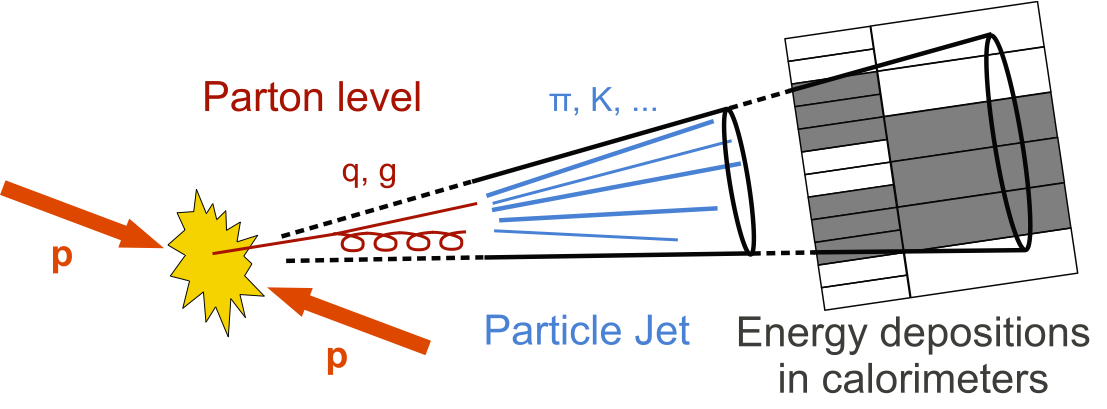
\includegraphics[width=0.5\linewidth, angle=0]{figs/Objects/jets_schem.png}
%  \end{center}
%   \vspace{-0.5em}
%  \caption[A schematic illustrating the formation of hadronic jets and the resulting observed energy deposits in the calorimeter system.]
%          {A schematic illustrating the formation of hadronic jets and the resulting observed energy deposits in the calorimeter system \cite{obj-jets_schem}.}
%          \label{fig:obj-jets_schem}
%          \vspace{-1em}
%\end{figure} 

This section describes the jet building procedure utilised by ATLAS
to convert energy deposits in calorimeter cells into well defined and calibrated hadronic jets.
Only hadronic jets built from calorimeter cells are described,
as this is the jet object used in di-$b$-jet searches.
Other types of jets used %at ATLAS
are, for example, jets constructed from tracks~\cite{obj-Hbb_exotic}.

\subsection{Hadronic Topocluster Reconstruction}
\label{sec:obj-jets_topo}

The first step of jet building at ATLAS is the formation of 3D clusters, known as topoclusters, from groups of energy deposits in neighbouring calorimeter cells~\cite{obj-jets_topo}.
Each topocluster represents a hadron or a set of collimated hadrons within a hadronic jet.
The calorimeter cells can be from either the EM or hadronic calorimeter systems which are described in Section~\ref{sec:det-calo}.
The topocluster building algorithm uses the variable \mbox{\textit{`cell signal significance'}}
, $S_{\text{cell}}$, defined as:
\begin{equation}
  \vspace{0.2em}
  {S_{\text{cell}} = \frac{E_{\text{cell}}}{\sigma_{\text{noise,cell}}}}
\end{equation}
where $E_{\text{cell}}$ is the energy deposited in a cell
and $\sigma_{\text{noise,cell}}$ is the background noise in a cell.
%The sources of noise in a calorimeter cell noise was described in Section~\label{sec:det-calo_noise}.
A value of $S_{\text{cell}} >$ 1 indicates that the energy deposit is likely due to a real particle rather than noise in the calorimeter.

\noindent
Using the value of $S_{\text{cell}}$, each calorimeter cell is labelled as follows
\vspace{-1em}
\begin{itemize}
\item If \ \ \ \ \ \ \ ($|S_{\text{cell}}| > 4$): the cell is labelled as a \textbf{seed} cell.
\item If ($2 < |S_{\text{cell}}| < 4$): the cell is labelled as a \textbf{growth} cell.
\item If ($0 < |S_{\text{cell}}| < 2$): the cell is labelled as a \textbf{boundary} cell.
\end{itemize}
Topoclusters are then built using the following steps
\vspace{-1em}
\begin{enumerate}
\item A seed cell forms the centre of a new topocluster.
\item Neighbouring seed cells are added together to form one topocluster seed.
\item Then, growth cells neighbouring the topocluster are added.
\item Finally, boundary cells neighbouring the topocluster are added.
\end{enumerate}
Figure~\ref{fig:obj-topo_schem} shows an illustration of a set of energy deposits that would form a topocluster
and a set of energy deposits that would not form a topocluster, as no seed cell is present.

\begin{figure}[!htb]
  \begin{center}
    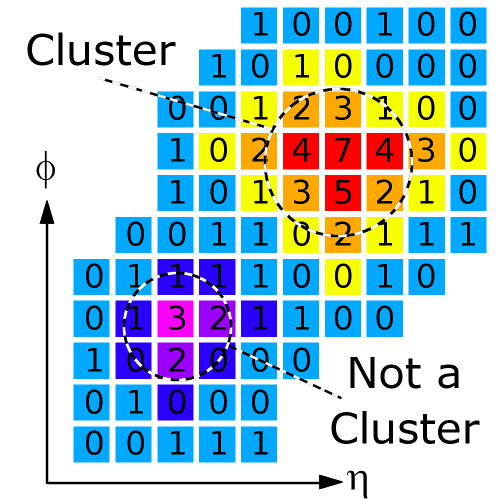
\includegraphics[width=0.5\linewidth, angle=0]{figs/Objects/topo_schem.png}
  \end{center}
  \caption[A schematic illustrating the algorithm used to form a topocluster.]
          {A schematic illustrating the algorithm used to form a topocluster. The numbers on the grid represent $|S_{\text{cell}}|$ and the colours represent the cell label~\cite{det-magnet_fig}.}
  \label{fig:obj-topo_schem}
\vspace{-0.2em}
\end{figure}

The topoclusters are treated as massless objects \footnote{\ As no particle identification is possible in the hadronic calorimeter an assumption of the mass is required.}
such that the four-momentum of each topocluster is determined from the $\eta-\phi$ position and the sum of energy deposited.
%The constructed topoclusters and their four-momenta are then used as the inputs to the next step of jet reconstruction.

\subsection{Jet Reconstruction}
\label{sec:obj-jets_reco}

In the next step of jet building, jet reconstruction algorithms are employed to build jets from
the four-momenta of the topoclusters.
Each jet built by the algorithm has a well defined four-momentum and set of constituents.
A detailed discussion of jet reconstruction algorithms is found in~\cite{obj-jets_reco_salam}.

ATLAS analyses use a type of jet reconstruction algorithm known as sequential recombination algorithms,
which selectively add together the calorimeter topoclusters to form the jet;
these are specifically the $k_t$, anti-$k_t$ and Cambridge-Aachen (CA) algorithms.
%The use of sequential recombination jet reconstruction algorithms means that the
%reconstructed jets are experimentally well-defined model-independent observables,
%which is required if measurements using jets are to be re-usable by the wider particle physics community.

The sequential recombination algorithms consider a set of four-momenta which are referred to as clusters;
the initial set of clusters are the topoclusters described above.
The algorithm makes use of two distances: the inter-jet distance between clusters $i$ and $j$ ($d_{ij}$) 
and the particle-beam distance for cluster $i$ ($d_{iB}$). The distances are defined as
\begin{equation}
  d_{ij} = \text{min}[(p_{ Ti})^a, (p_{ Tj})^a]  \left(\frac{\Delta  R_{ij}}{R}\right) ^2, \hspace{1cm}  d_{iB} = (p_{Ti})^a  \label{dij}
\end{equation}
%\begin{equation}
%  d_{ij} = \text{min}
%  [(p_{ Ti})^a, (p_{ Tj})^a]  \left(\frac{\Delta  R_{ij}}{R}\right) ^2, \hspace{1cm} \Delta R_{ij} = \sqrt{(y_{i} - y_{j})^2 + (\phi_{i} - \phi_{j})^2} \label{dij}
%\end{equation}
%\noindent and a particle-beam distance for cluster $i$ defined as,
%\begin{equation}
%  d_{iB} = (p_{Ti})^a \label{diB}
%\end{equation}
where \pT{} is transverse momentum (component of momentum perpendicular to the beam-pipe)
and $\Delta R_{ij} = \sqrt{(y_{i}-y_{j})^2 + (\phi_{i}-\phi_{j})^2}$.
$R$ is the jet width parameter, a free parameter of the algorithm.
The parameter $a$ takes the value $a = 2$ for the $k_t$ algorithm, $a = -2$ for the anti-$k_t$ algorithm 
and  $a = 0$ for the Cambridge-Aachen algorithm.
If $d_{ij} < d_{iB}$ for a pair of clusters then it is likely that the two clusters are from the same jet. 
In contrast, if $d_{ij} > d_{iB}$ then it is unlikely that the two clusters are from the same jet.

%The three algorithms use a set of four-momenta (clusters), which are initially the topoclusters formed in the calorimeter.
%One then introduces an inter-jet distance between clusters $i$ and $j$ defined as,
%\begin{equation}
%  d_{ij} = \text{min}
%  [(p_{ Ti})^a, (p_{ Tj})^a]  \left(\frac{\Delta  R_{ij}}{R}\right) ^2, \hspace{1cm} \Delta R_{ij} = \sqrt{(y_{i} - y_{j})^2 + (\phi_{i} - \phi_{j})^2} \label{dij}
%\end{equation}
%\noindent and a particle-beam distance for cluster $i$ defined as,
%\begin{equation}
%  d_{iB} = (p_{Ti})^a \label{diB}
%\end{equation}
%where $y$  is rapidity (as defined in Section~\ref{sec:det-coordinate}), $\phi$ is azimuthal angle,
%\pT{} is transverse momentum (component of momentum perpendicular to the beam-pipe of colliding particles)
%and $p_z$ is the component of momentum that is parallel to the beam-pipe of colliding particles.
%$R$ is the jet width parameter, a free parameter of the algorithm.
%The parameter $a$ in Eq. \eqref{dij} and \eqref{diB} takes the value $a = 2$ for the $k_t$ algorithm, $a = -2$ for the anti-$k_t$ algorithm 
%and  $a = 0$ for the Cambridge-Aachen algorithm.
%$d_{ij}$ and $d_{iB}$ are not physical distances, but are instead dimensional measures of how likely it is that
%clusters $i$ and $j$ represent clusters caused by hadrons from the same jet.

\newpage
\noindent Sequential reclustering algorithms then proceed using the following steps:
\vspace{-1em}
\begin{enumerate}[nolistsep,leftmargin=*]
  \item Calculate $d_{ij}$ and $d_{iB}$ for all combinations of clusters and find the minimum.
  %\item Find the minimum of the $d_{ij}$ and $d_{iB}$.
  \item If the minimum is a $d_{ij}$ combine cluster $i$ and $j$ to form a new cluster. 
  \item If the minimum is a $d_{iB}$ declare cluster $i$ as a final-state jet and remove it from the set.  
  \item Repeat until all clusters have been declared as final-state jets. 
\end{enumerate} 

The four-momentum of a final-state jet is the sum of the four-momenta of the topoclusters assigned to that jet.
The jet width parameter, $R$, effectively gives the maximum width of a reconstructed jet
because if $\Delta R_{ij} > R$  for a pair of clusters then
$d_{iB} < d_{ij}$ for one of the clusters %(depending on the value of $a$)
and so the two cluster cannot be merged.

The sequential reclustering algorithms described above are used as they satisfy two important %theoretically motivated
criteria: infrared and collinear safety \footnote{\ Cone-based jet reconstruction algorithms used at some previous collider experiments,
  such as UA2 ~\cite{obj-jets_reco_UA2}, do not satisfy infrared and collinear safety.}.
Infrared safety requires that the jet reconstruction algorithm result should be invariant against soft gluon emission \footnote{\ Soft means low momentum.}
and collinear safety requires that the result should be invariant against a parton splitting into two partons with small angular separation.
If the jet reconstruction algorithm is not infrared and collinear safe,
two different sets of jets could be built from identical hard-scatter processes
due to an additional emission process in the parton shower.

Anti-$k_T$ is the standard jet reconstruction algorithm used at ATLAS. %, which is typical of analyses at ATLAS.
This is because the anti-$k_T$ algorithm provides regular jet shapes around the centre of the jet as
the algorithm reconstructs the high-\pT{} core of the jets first and then adds in the lower \pT{} suburbs. % in later steps.
To illustrate this point, Figure~\ref{fig:obj-jets_reco_shapes} shows the jets built by the %Cambridge-Aachen,
$k_T$ and anti-$k_T$ algorithm using the same set of input clusters; the anti-$k_T$ algorithm creates a more regular jet shape.
%this illustrates that anti-$k_T$ algorithm creates more regular jet shapes than the other sequential-reclustering algorithms.

 \begin{figure}[!ht]
  \captionsetup[subfigure]{aboveskip=-5pt,justification=centering}
  \begin{center}
    %\subcaptionbox{Cambridge-Aachen} {
    %  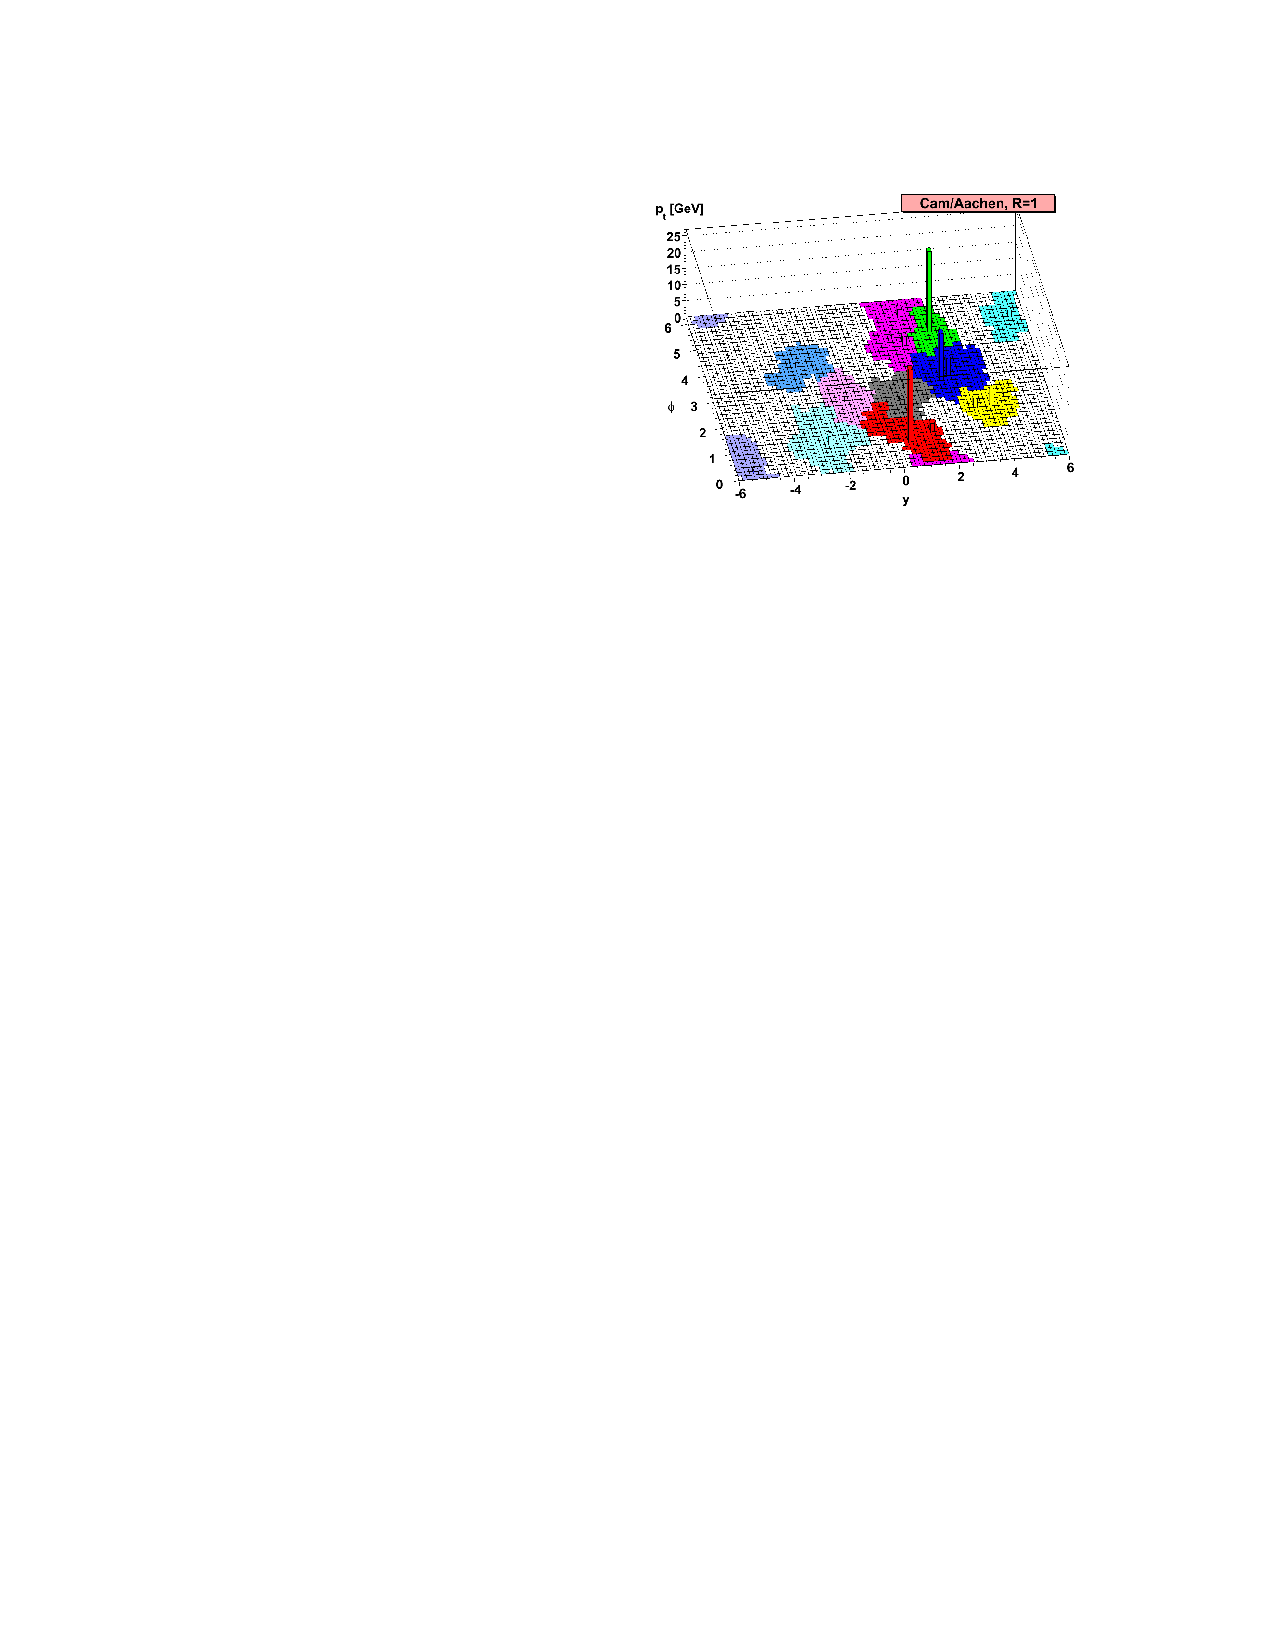
\includegraphics[width=0.45\linewidth, angle=0]{figs/Objects/jets_reco_shapes_ca.pdf}
    %}
    \subcaptionbox{$k_T$} {
      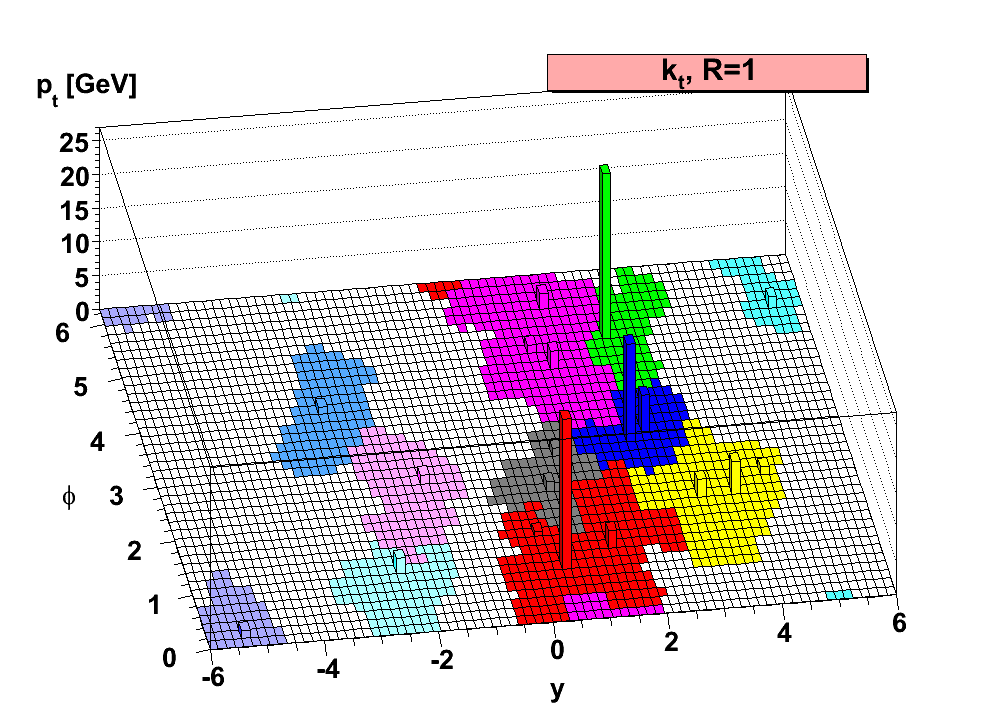
\includegraphics[width=0.45\linewidth, angle=0]{figs/Objects/jets_reco_shapes_kt.png}
    }%\\
    \subcaptionbox{Anti-$k_T$} {
      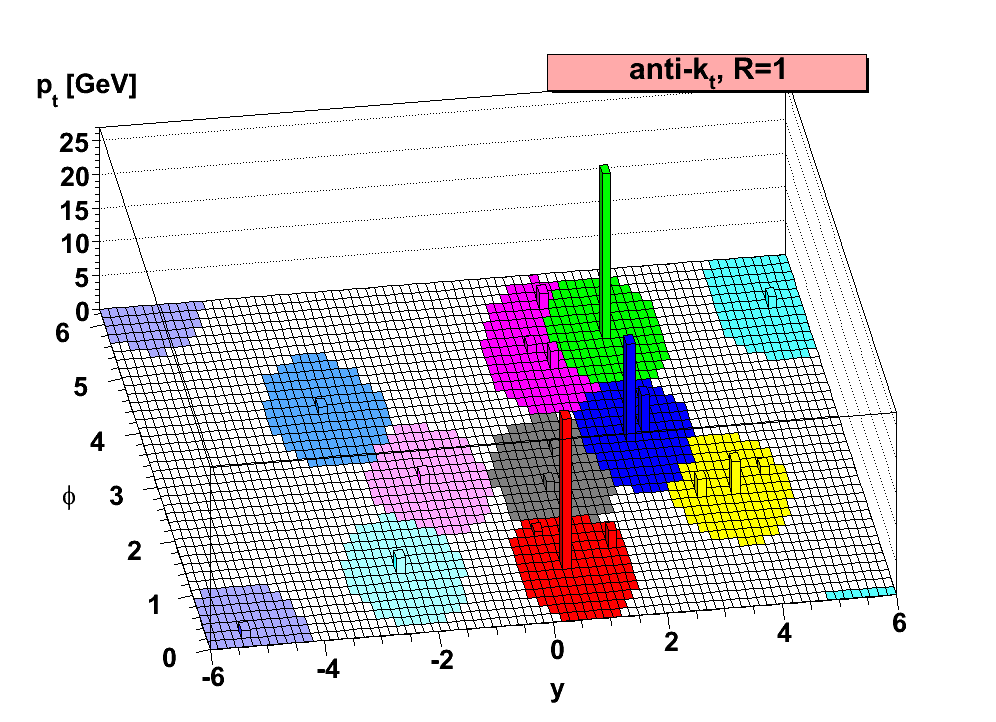
\includegraphics[width=0.45\linewidth, angle=0]{figs/Objects/jets_reco_shapes_akt.png}
    }

  \end{center}
  \caption[A comparison of the jets built using the $k_T$ and anti-$k_T$ algorithm.]
          {A comparison of the jets built using the (a) $k_T$ and (b) anti-$k_T$ algorithm from the same simulated event.
            The constituent clusters of each of the jets built is indicated using various colours \cite{obj-jets_reco_akt}.}
          %\caption[A comparison of the jets built using the (a) Cambridge-Aachen, (b) $k_T$ and (c) anti-$k_T$ algorithm from the same simulated event.
          %  The constituent clusters of each of the jets built is indicated using various colours.]
          %        {A comparison of the jets built using the (a) Cambridge-Aachen, (b) $k_T$ and (c) anti-$k_T$ algorithm from the same simulated event.
          %          The constituent clusters of each of the jets built is indicated using various colours \cite{obj-jets_reco_akt}.}
  \label{fig:obj-jets_reco_shapes}
\end{figure}

%To choose the jet width parameter, $R$, one must balance the effects that the
%momentum of a narrow jet can be greatly changed by an additional gluon emission in the parton shower process
 %whilst the momentum of a wide jet is greatly affected by the underlying event \footnote{\  Underlying event means objects from either the remnants of the proton from the hard-scatter or pile-up.}.
To choose the jet width parameter, $R$, one must balance the effects that
a narrow jet will not contain all the energy from the jet formation process
whilst a wide jet will include energy from the underlying event.
%\footnote{\  Underlying event means objects from either the remnants of the proton from the hard-scatter or pile-up.}.
The standard choice at ATLAS is $R$=0.4 to minimise the  two effects described above;
Section 5 of~\cite{obj-jets_reco_salam} provides a numerical calculation to justify this choice.


\subsection{Jet Calibration}
\label{sec:obj-jets_calib}

The jets initially built from the topoclusters will not represent the true energy of the hadronic jet.
%and as such will not give an accurate dijet mass reconstruction which is required for the analyses presented in this thesis.
The key factors for the unrepresentative hadronic jet energy measurement are~\cite{det-thesis_kate,obj-jets_calib_2015}:
\begin{itemize}[leftmargin=*]
\item\textbf{Jet Energy Scale}:
  As discussed in Section~\ref{sec:det-calo_HCAL}, the response of the ATLAS calorimeter is different for an EM-object and a hadronic object.
  The calorimeter energy response is initially calibrated for an EM-object.
  Therefore energy measurements of hadronic objects must be corrected using a jet energy scale correction. \vspace{0.5em}
\item\textbf{Detector Effects}:
  Some of the jet energy may be deposited either in an inactive region within the ATLAS detector,
  outside of the angular acceptance of the calorimeter or beyond the calorimeter, an effect known as `punch-through'.\vspace{0.5em}
\item\textbf{Jet Reconstruction}:
  Jet energy can be lost either in topocluster formation due to the cell signal significance thresholds
  or from inaccuracies in the jet reconstruction algorithm.\vspace{0.5em}
\item\textbf{Pile-Up}:
  In Section~\ref{sec:det-LHC} pile-up was defined as proton collisions other than the hard-scatter primary vertex.
  Particles from pile-up collisions can be included in the jet reconstruction and hence effect the jet energy measurement.
  %This includes in-time and out-of-time pile-up.
  %A  definition of pile-up can be found in Section~\cite{}. 
\end{itemize}
\vspace{-0.5em}
As a result, a calibration procedure is performed to correct the energy of a jet~\cite{obj-jets_calib_run2}.

For a calibration, one must decide what to correct with respect to.
Naively one could choose the truth initial parton,
however the correction would then strongly depend on the theoretical modelling of the parton shower and hadronisation process.
The resulting corrected jets would then not be model-independent~\footnote{\ An explanation of why model-independent jets are desirable is found in~\cite{theo-jets_jb}.}.
Instead, jets are corrected with respect to a `truth jet';
where a truth jet is constructed by running the anti-$k_T$ algorithm on the set of stable truth particles in a simulated event.
A stable particle is required to have a lifetime $c\tau >$ \SI{10}{\milli\metre} and muons, neutrinos, and particles from pile-up collisions are ignored.
Truth jets are a good choice as they are well-defined and model-independent objects representing the jets that would have been reconstructed if one had a perfect detector.

\newpage
The calibration process uses Monte-Carlo simulation and data to correct the jets initially
built from the EM-scale topoclusters using a number of steps: \vspace{-0.5em}

%These steps are outlined in Figure~\ref{fig:obj-jets_calib_schem}.
%\begin{figure}[!htb]
%  \begin{center}
%    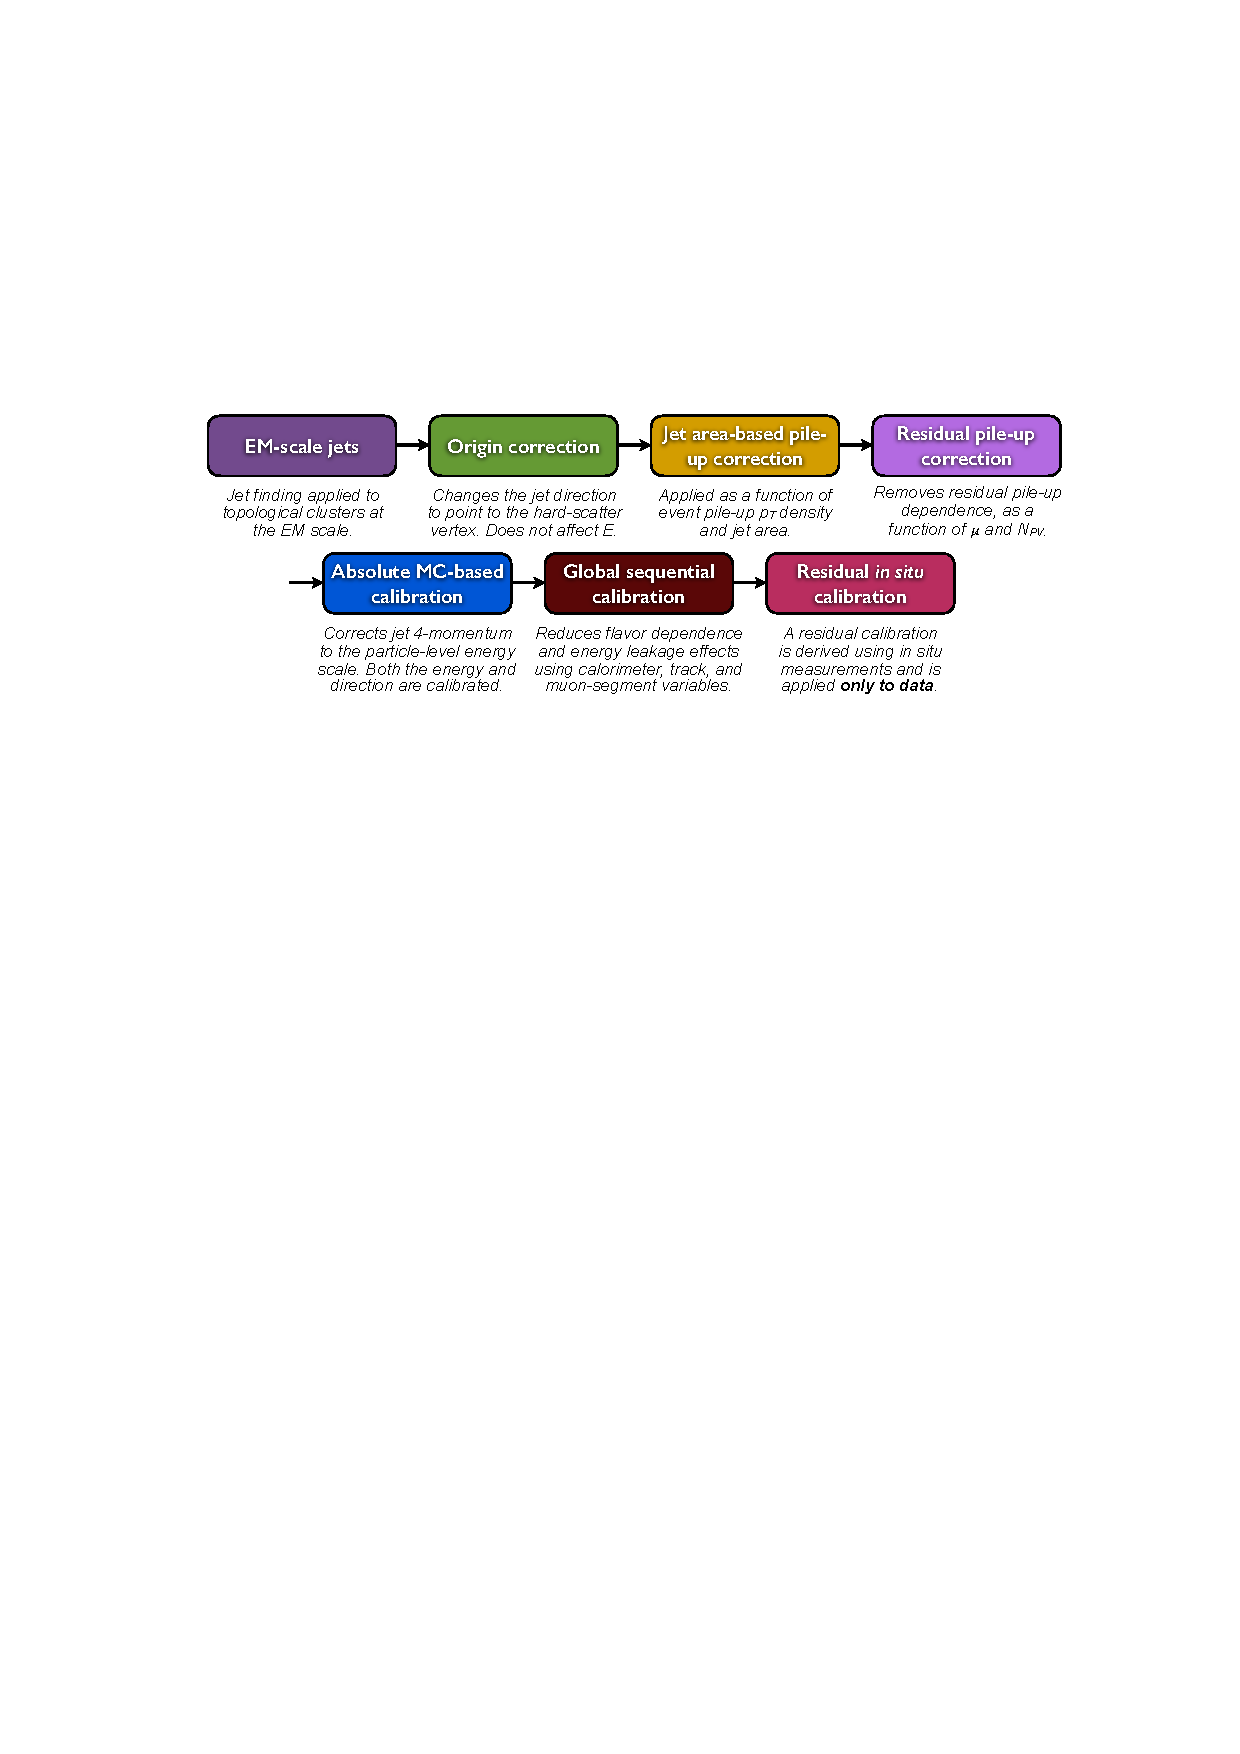
\includegraphics[width=0.9\textwidth]{figs/Objects/jets_calib_schem.pdf}
%    \caption[Calibration stages for the EM+JES calibration scheme.]
%            {Calibration stages for the EM+JES calibration scheme~\cite{obj-jets_calib_run2}.}
%    \label{fig:obj-jets_calib_schem}
%  \end{center}
%  \vspace{-0.5cm}
%\end{figure}
%\noindent
%To discuss each step in a little more detail:
%\vspace{-0.5em}
\begin{enumerate}[leftmargin=*]
\item\textbf{Origin Correction}:
  This step changes the direction of the jets such that the four-momentum is pointing at the hard-scatter primary vertex
  rather than the centre of the detector.
  This calculation conserves the jet energy.\vspace{0.3em}
\item\textbf{Jet Area-Based Pile-Up Correction}:
  This step removes unwanted energy contributions from pile-up.
  This correction subtracts the area of the jet, $A$, multiplied by the average energy density due to pile-up, $\rho$.
  $\rho$ is calculated for each event using the median $(\pT/A)$ of a set of jets reconstructed
  from positive-energy topo-clusters in the range $|\eta| <$ 2
  using the $k_T$ algorithm with $R$ = 0.4.\vspace{0.3em}
\item\textbf{Residual Pile-Up Correction}:
  This step further reduces effects from pile-up utilising the linear dependence of pile-up effects on
  the number of primary vertices, $N_{\text{PV}}$,
  and the mean number of $pp$ collisions per bunch crossing, $<\hspace{-3pt}\mu\hspace{-3pt}>$.
  This correction can hence be written as \hspace{2mm}$\pT^{\text{Pile-up Corrected}} = \pT^{\text{Initial}}  - \alpha * (N_{PV}-1) - \beta * \mu\,$,\hspace{2mm}
  where $\alpha$ and $\beta$ are constants derived using simulated events. \vspace{0.3em}
  %%% Does not depend on A:
  % pcorr = preco −ρ×A−α×(NPV −1)−β×μ,
  % my feeling is that alpha and beta implicitly includes A as they are fitted quantaties.
  % Alpha is derevied (eta and phi)

  %\\
  %\vspace{1em}
  %Therefore, the combination of Steps 2 and 3 can be rewritten as: \vspace{-1.5em}
  %\begin{equation}
  %\pT^{\text{Pile-up Corrected}} = \pT^{\text{Inital}} - \rho * A - \alpha * (N_{PV}-1) - \beta * \mu
  %\vspace{-0.5em}
  %\end{equation}   
  %where $\alpha$ and $\beta$ are constants derived using simulated events.\\

\item\textbf{Absolute JES Correction}:
  This step corrects the jet four-momentum from the EM-scale, at which they were initially built, to the truth jet energy.
  This correction is derived using truth jets and reconstructed jets in Monte-Carlo simulated dijet events.\vspace{0.3em}
\item\textbf{Global Sequential Calibration}:
  This step uses information from the calorimeter, muon spectrometer and track-based variables
  to refine the reconstructed energy and reduce the overall uncertainties.\vspace{0.3em}
\item\textbf{In-situ calibration}:
  All previous steps use simulation to correct detector-level jets to truth jets.
  This step corrects for differences between simulation and data using events
  containing a jet to be calibrated and a reference object;
  the reference object is a photon, a $Z$ boson, or a set of calibrated jets.
  The reference objects used have been calibrated such that they have a well measured $\pT$;
  therefore, from conservation of momentum, the true \pT{} of the jet to be calibrated can be inferred.
  One can then calculate a correction factor, which is applied to the jet four-momentum in data only.
  \begin{equation}
    %\text{Correction} = \frac{1}{R(p_T, \eta)} = \frac{ < p_T^{\text{jet}}/p_T^{\text{ref}}>_{\text{MC}} }{ < p_T^{\text{jet}}/p_T^{\text{ref}}>_{\text{Data}} }
    \text{Correction Factor}~(p_T, \eta) = \frac{ < p_T^{\text{jet}}/p_T^{\text{ref}}>_{\text{MC}} }{ < p_T^{\text{jet}}/p_T^{\text{ref}}>_{\text{Data}} }
  \end{equation}
  %; this correction is not applied in simulation.
\end{enumerate}

This calibration scheme is called `EM+JES', as the topoclusters are at the EM-scale.
There are other schemes used for calibrating jets at ATLAS,
for example, some analyses~\cite{obj-VVjj} correct each topocluster to the hadronic scale
before clustering the jet, in a scheme called Local Cluster Weighted (LCW)~\cite{obj-jets_topo}.
EM+JES is generally used in ATLAS analyses as it is a simpler calibration scheme than LCW, but provides similar results.

%\newpage
The end result of the processes described in this section is a jet
reconstructed from EM-scale topoclusters using an anti-$k_T$ algorithm with a jet width parameter $R$=0.4
that is calibrated using the EM+JES calibration scheme.
This is the definition of a jet used throughout this thesis.

\subsection{Jet Energy Uncertainties}
\label{sec:obj-jets_uncert}

There are two components of uncertainty on the jet energy measurement; jet energy scale and jet energy resolution.

Jet energy scale (JES) uncertainties arise from the calibration procedure
to correct jets from the EM-scale to the hadronic-scale, outlined above.
80 separate uncertainties are derived to cover each step of the calibration,
the dominant uncertainties arise from the data-driven in-situ step~\cite{obj-jets_calib_run2}.
Figure~\ref{fig:obj-jets_calib_JES} shows the fractional JES uncertainty as a function of jet-\pT{} and jet-$\eta$.
The increased uncertainty in the region $2 < |\eta| < 2.6$ is caused by localised data/simulation discrepancies
caused by mismodelling of the detector response in the EM end-cap calorimeters.

\begin{figure}[!htb]
  \begin{center}
    \captionsetup[subfigure]{aboveskip=0pt,justification=centering}
    \subcaptionbox{Jet-\pT{}} {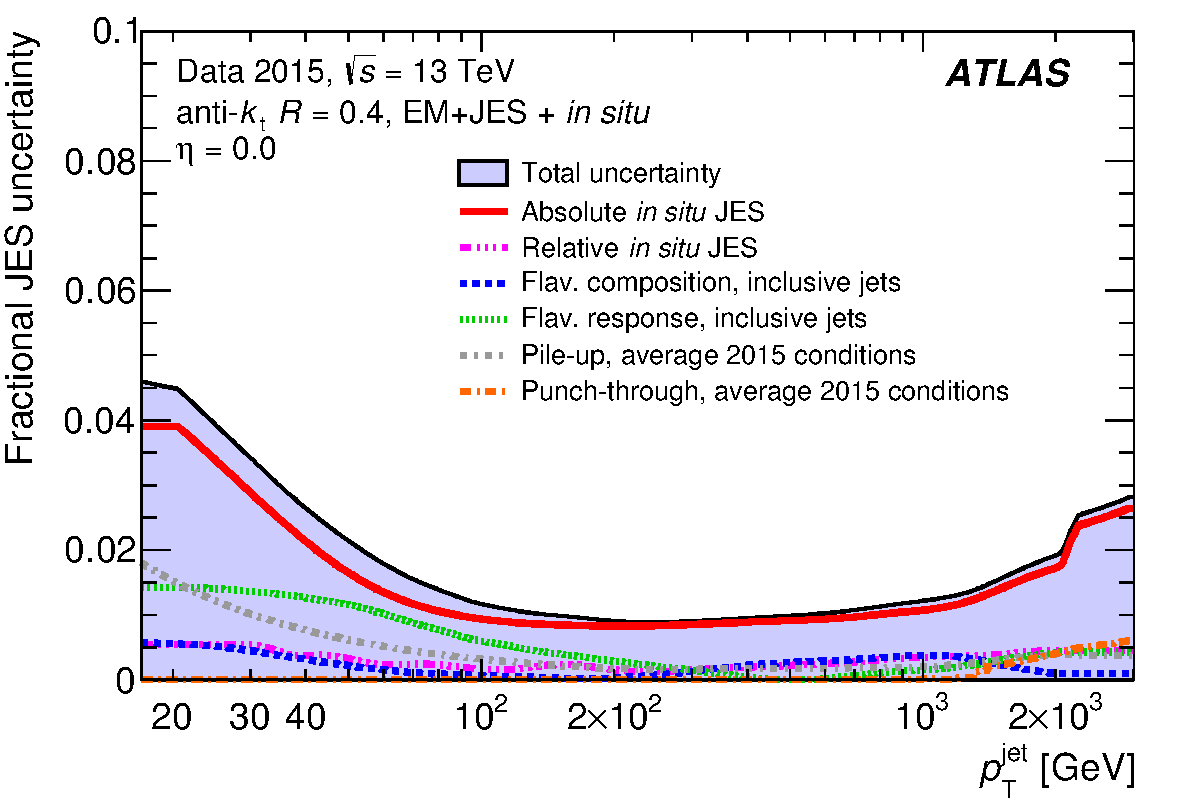
\includegraphics[width=0.55\linewidth, angle=0]{figs/Objects/jets_uncert_JES_pt.pdf} }
    \subcaptionbox{Jet-\eta}{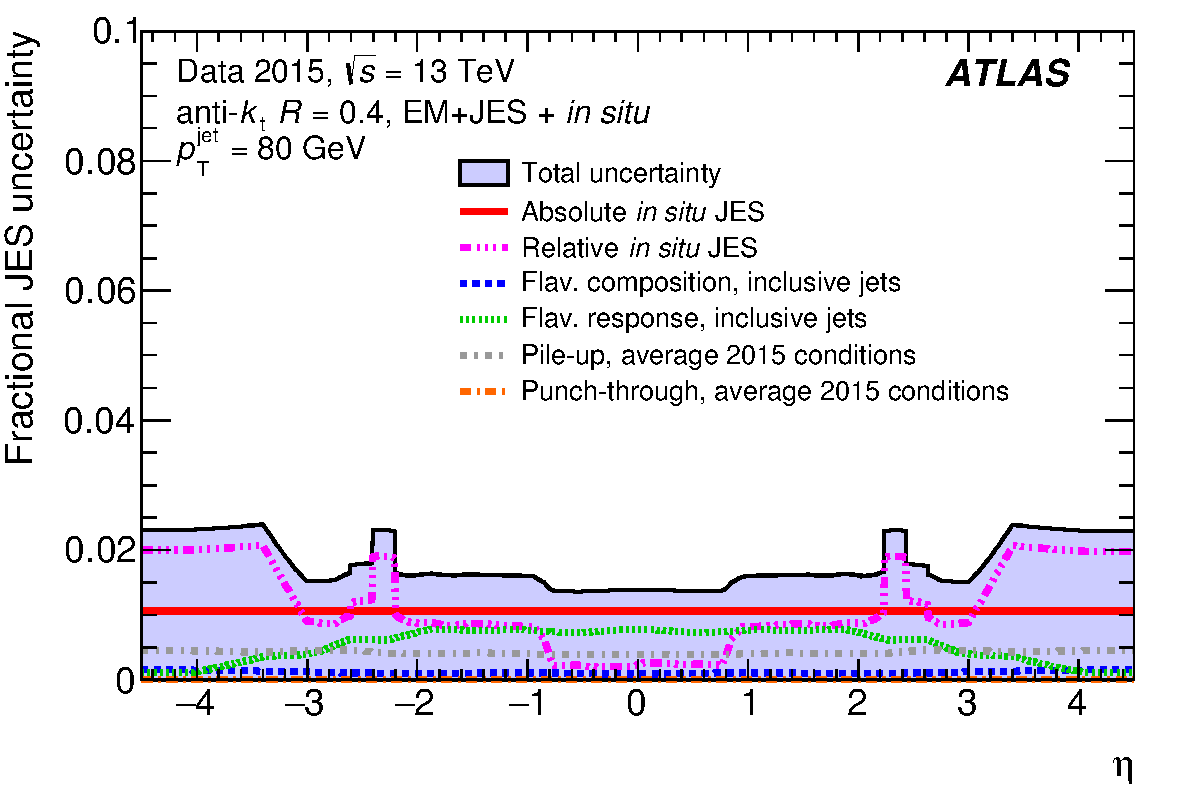
\includegraphics[width=0.55\linewidth, angle=0]{figs/Objects/jets_uncert_JES_eta.pdf} }
  \end{center}
 \vspace{-1em}
  \caption[The fractional jet energy scale uncertainty as a function of jet-\pT{} and \eta.]
          { \label{fig:obj-jets_calib_JES} The fractional jet energy scale uncertainty as a function of jet-\pT{} and \eta.
            The total uncertainty is shown with the contributions from the various sources of uncertainty~\cite{obj-jets_calib_run2}.}
\end{figure}

Jet energy resolution (JER) is defined as $\sigma(E)/E$, and JER uncertainties
account for the imperfect simulation of detector resolution in Monte-Carlo simulation.
The uncertainty is measured using an in-situ technique from the balancing of jets in 8 TeV collision data
which is extrapolated for 13 TeV data; the final uncertainty accounts for this extrapolation.
Figure~\ref{fig:obj-jets_calib_JER} shows the fractional JER uncertainty as a function of jet-\pT{} and jet-$\eta$.
Full details on the derivation of this uncertainty can be found in~\cite{obj-jets_calib_2015}~and~\cite{obj-jets_calib_JER_8TeV}.

\begin{figure}[!htb] 
 \vspace{0.2em}
  \begin{center}      
    \captionsetup[subfigure]{aboveskip=0pt,justification=centering}
    \subcaptionbox{Jet-\pT{}} {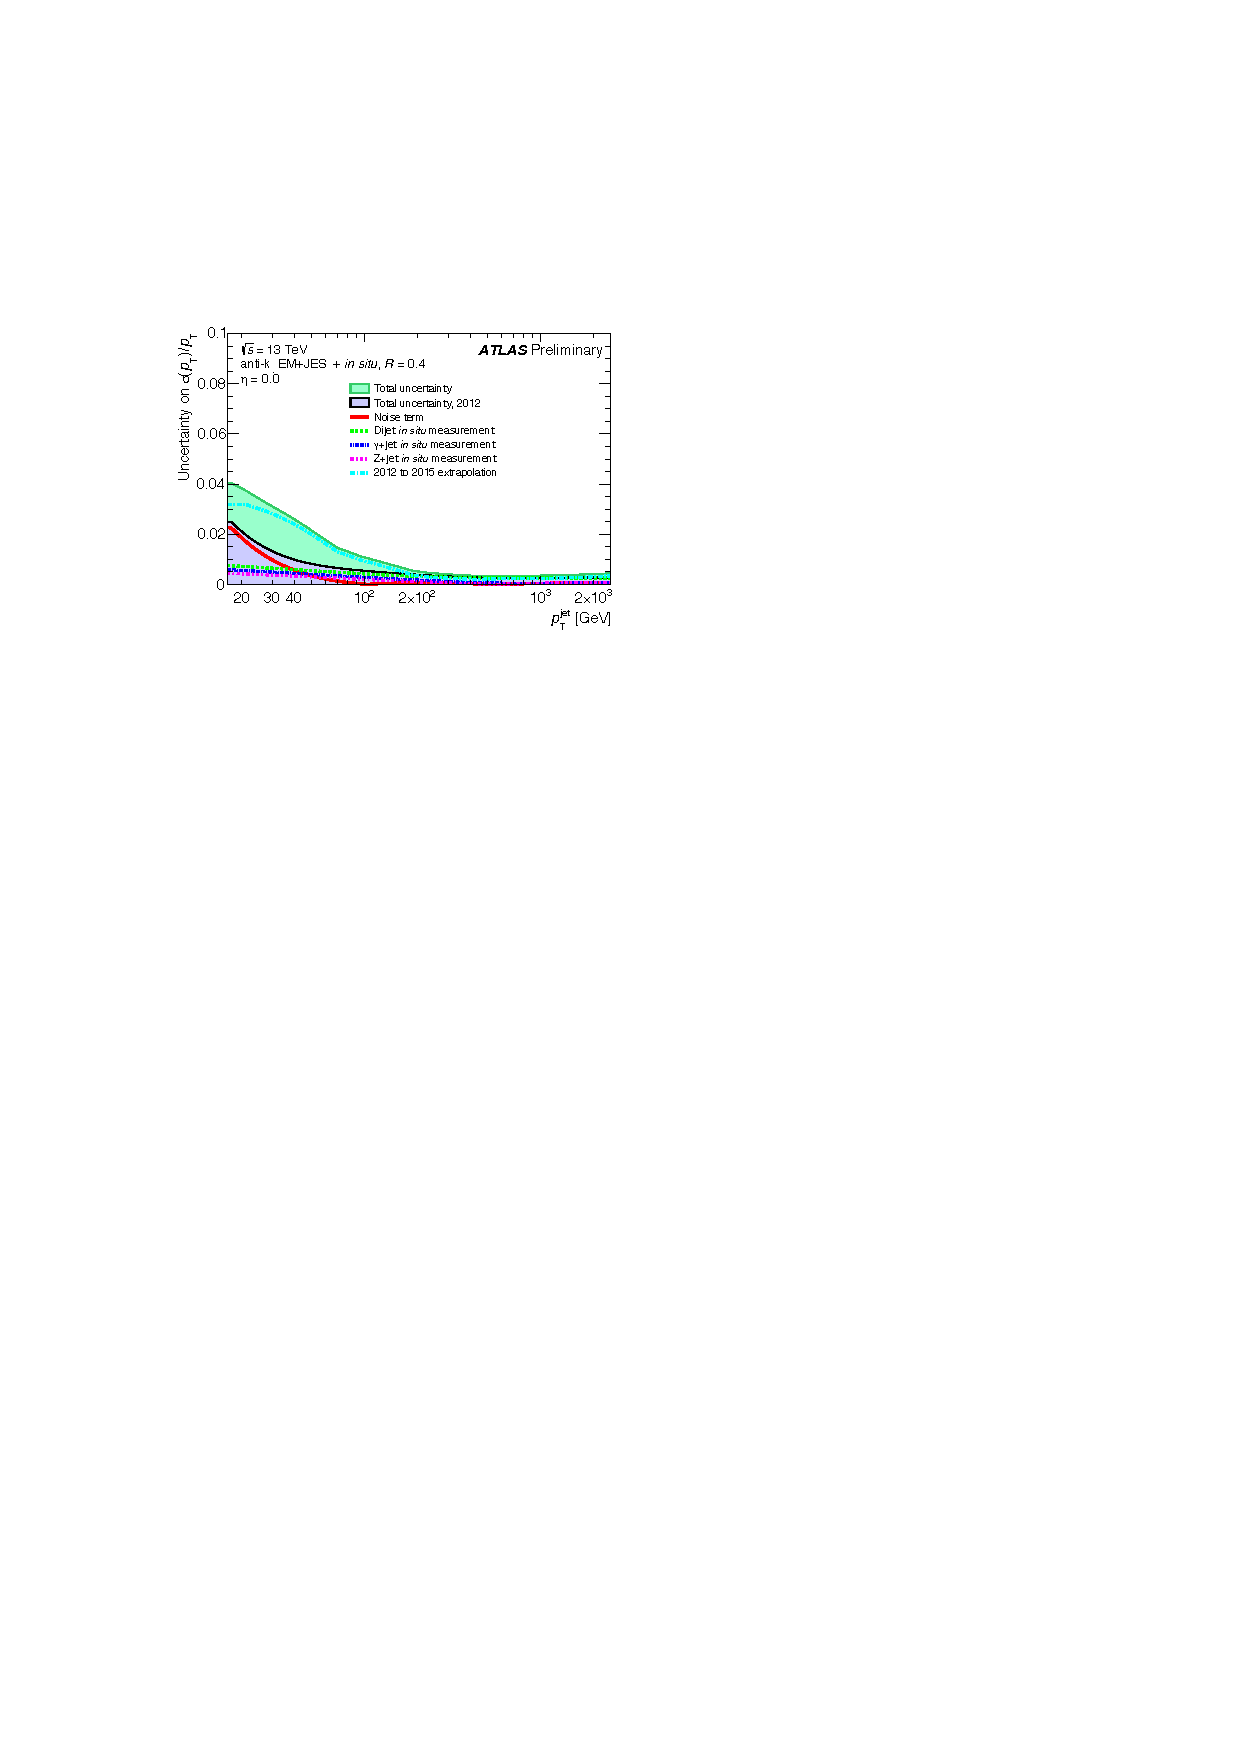
\includegraphics[width=0.6\linewidth, angle=0]{figs/Objects/jets_uncert_JER_pt.pdf} }
    \subcaptionbox{Jet-\eta}{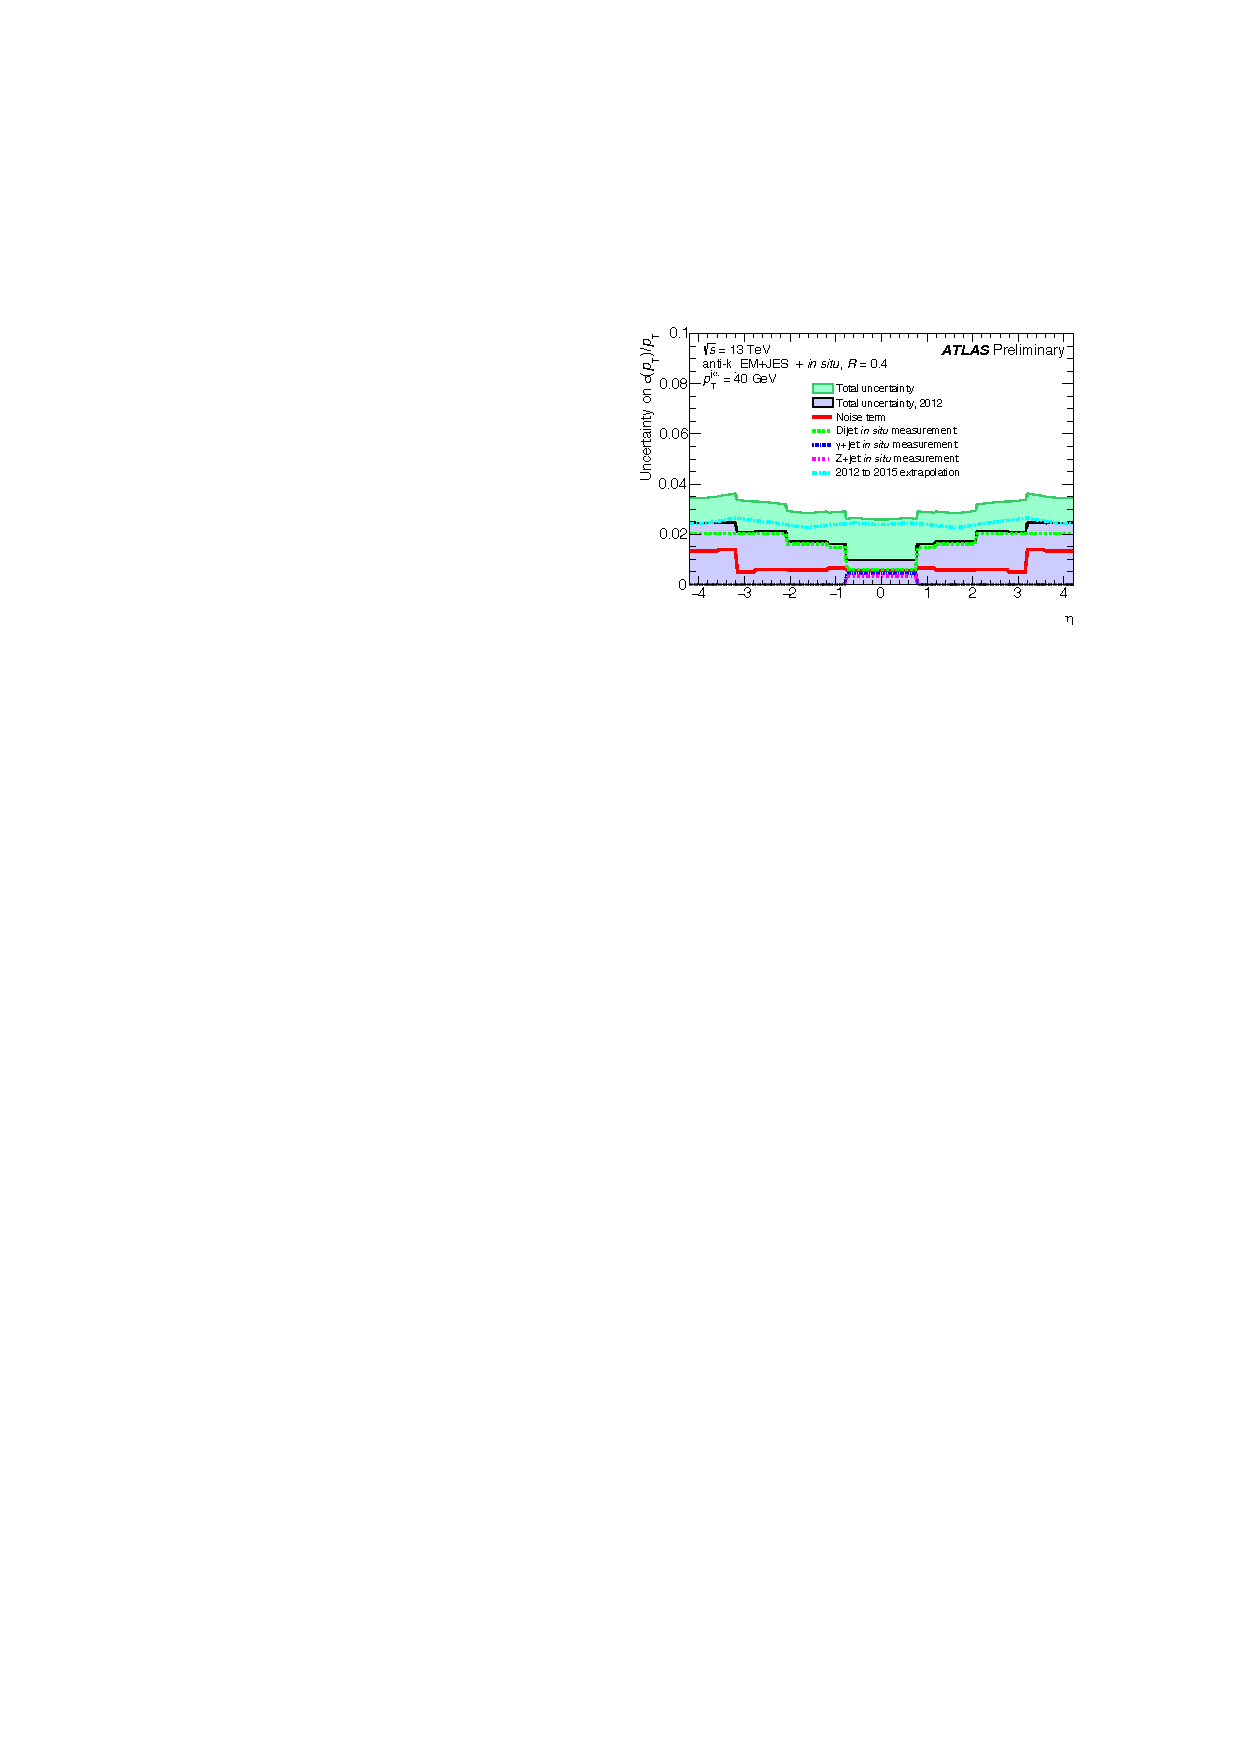
\includegraphics[width=0.6\linewidth, angle=0]{figs/Objects/jets_uncert_JER_eta.pdf} }
 \end{center}
 \vspace{-1em}
  \caption[The fractional jet energy resolution uncertainty as a function of jet-\pT{} and \eta.]
          {\label{fig:obj-jets_calib_JER} The fractional jet energy resolution uncertainty as a function of jet-\pT{} and \eta.
            The total uncertainty is shown with the contributions from the various sources of uncertainty~\cite{obj-jets_calib_2015}.}
\end{figure}

\clearpage

\section{$b$-Jets}
\label{sec:obj-bjets}

There are three flavour categories of hadronic jets based on the flavour of the constituent quarks.
$b$-jets are defined as jets containing one or more $b$-hadrons, where a $b$-hadron is any hadron containing a $b$-quark.
$c$-jets are defined as jets containing one or more $c$-hadrons but no $b$-hadrons
and light jets consist of only light hadrons (formed of $u$, $d$ and $s$ quarks).
%A description of how this definition is practically used in simulation is given in Section~\ref{sec:obj-bjets_label}.

The identification of $b$-jets, known as $b$-tagging, is an essential tool in a range of ATLAS collaboration results~\cite{obj-ttbar,obj-Hbb};
%for example analyses studying the $t\bar{t}$ final state \cite{obj-ttbar}
%\footnote{\ Section~\ref{sec:trig-bjet_eff} contains an analysis utilising $b$-tagging in the $t\bar{t}$ final state.}
%and the first direct evidence of the Higgs boson coupling to the quark-sector~\cite{obj-Hbb}.
%In the former, as the top decays to a \textit{W}-boson and a $b$-quark with a branching ratio close to 100\%, 
%the application of $b$-tagging can be used increase purity, this is used in the study described in Section~\ref{sec:trig-sys}.
%In the latter, the Higgs boson coupling is proportional to mass squared, hence the large mass of the
%$b$-quark means that $H\to b\bar{b}$ is the decay of the Higgs boson with the largest branching-ratio
%which means that it is the best channel to make the first direct observation of the Higgs boson coupling to fermions.
$b$-tagging is used in di-$b$-jet searches to reduce the light jet dominated background and increase 
sensitivity to BSM models that decay preferentially to 1 or 2 $b$-jets in their final state.

The process of $b$-tagging at ATLAS in Run-2 is described in great
detail in~\cite{obj-bjets_algo_2015,obj-bjets_algo_2016},
so what follows is a summary of the key features of the process.

\subsection{Truth Flavour Label}
\label{sec:obj-bjets_label}

In simulation, the particle-level truth information is known, and hence a truth flavour label of a jet can be defined.
Truth-level hadrons with $p_{T} >$ 5 GeV are matched to jets if $\Delta R <$ 0.3 between the reconstructed jet and the hadron;
the matching is exclusive meaning each hadron is assigned to the jet with the smallest $\Delta R$ separation.
If a $b$-hadron is matched to a jet, the jet is then declared a $b$-jet;
this process is then repeated for $c$-hadrons and $\tau$ leptons.
If no match between $b$, $c$ or $\tau$ is achieved, the jet is labelled as a light jet.
%The matching is exclusive, which means that each particle is only assigned to one jet.
This definition of truth flavour label in simulation is used generally within this thesis.

   
\subsection{Baseline $b$-Tagging Algorithms}
\label{sec:obj-bjets_base}

To identify $b$-jets in data, $b$-tagging algorithms utilise the long lifetimes of the heavy-hadrons that decay through the flavour changing weak interaction.
Weakly decaying $b$-hadrons produced at the LHC have an average lifetime of $\sim$\SI{1.6}{\pico\second} ~\cite{obj-bjets_PDG}
 \footnote{\ There are also excited $b$-hadron states that decay rapidly to other $b$-hadrons through the strong force.}.
A $b$-jet decay chain  will typically contain two of these flavour changing interactions 
as, at the quark level, the $b$-quark contained in the jet will decay to a $c$-quark, which will then decay into a $s$ or $d$ quark.
Due to their long lifetimes, $b$-hadrons decay a measurable distance from the hard-scatter primary vertex;
for example, a $B_0$ meson with a \pT{} of $100$ GeV will travel approximately $10$ mm.
%Note to laurie - First year talk contains this calc
%   p = gamma m v
%   d = vt = v gamma tau
%   d = p tau / m
%   Plug in numbers.
Hence, the flavour of a jet can be inferred from the presence of particles
that originate from a point offset from the hard-scatter primary vertex.

The $b$-tagging algorithms use tracks and jets as described in Section~\ref{sec:obj-tracks} and \ref{sec:obj-jets}.
To perform $b$-tagging, tracks are associated to jets if there is a small angular separation, $\Delta R$, between the two objects.
Tracks are exclusively matched, meaning each track is only associated to the jet with the smallest $\Delta R$ separation.
The maximum value of $\Delta R$ for association decreases as jet-\pT{} increases because high-\pT{} jets are more collimated;
$\,\Delta R_{\text{max}}$ is 0.45 for a jet-\pT{} of 20 GeV whilst $\,\Delta R_{\text{max}}$ is 0.26 for a jet-\pT{} of 150 GeV.

Three baseline $b$-tagging algorithms are utilised to produce flavour discriminating variables~\cite{obj-bjets_algo_2016}, which are described in the next three sections.
%Sections~\ref{sec:obj-bjets_IP}~to~\ref{sec:obj-bjets_JF}.
The flavour discriminating variables are then combined in a multi-variate algorithm described in Section~\ref{sec:obj-bjets_MV2}.
Figure~\ref{fig:obj_bjets_schem} shows a schematic illustrating how tracks
are used by the baseline $b$-tagging algorithms to identify a $b$-jet,
the details of this figure are referred to in the following three sections.

\begin{figure}[!htb]
  \begin{center}
    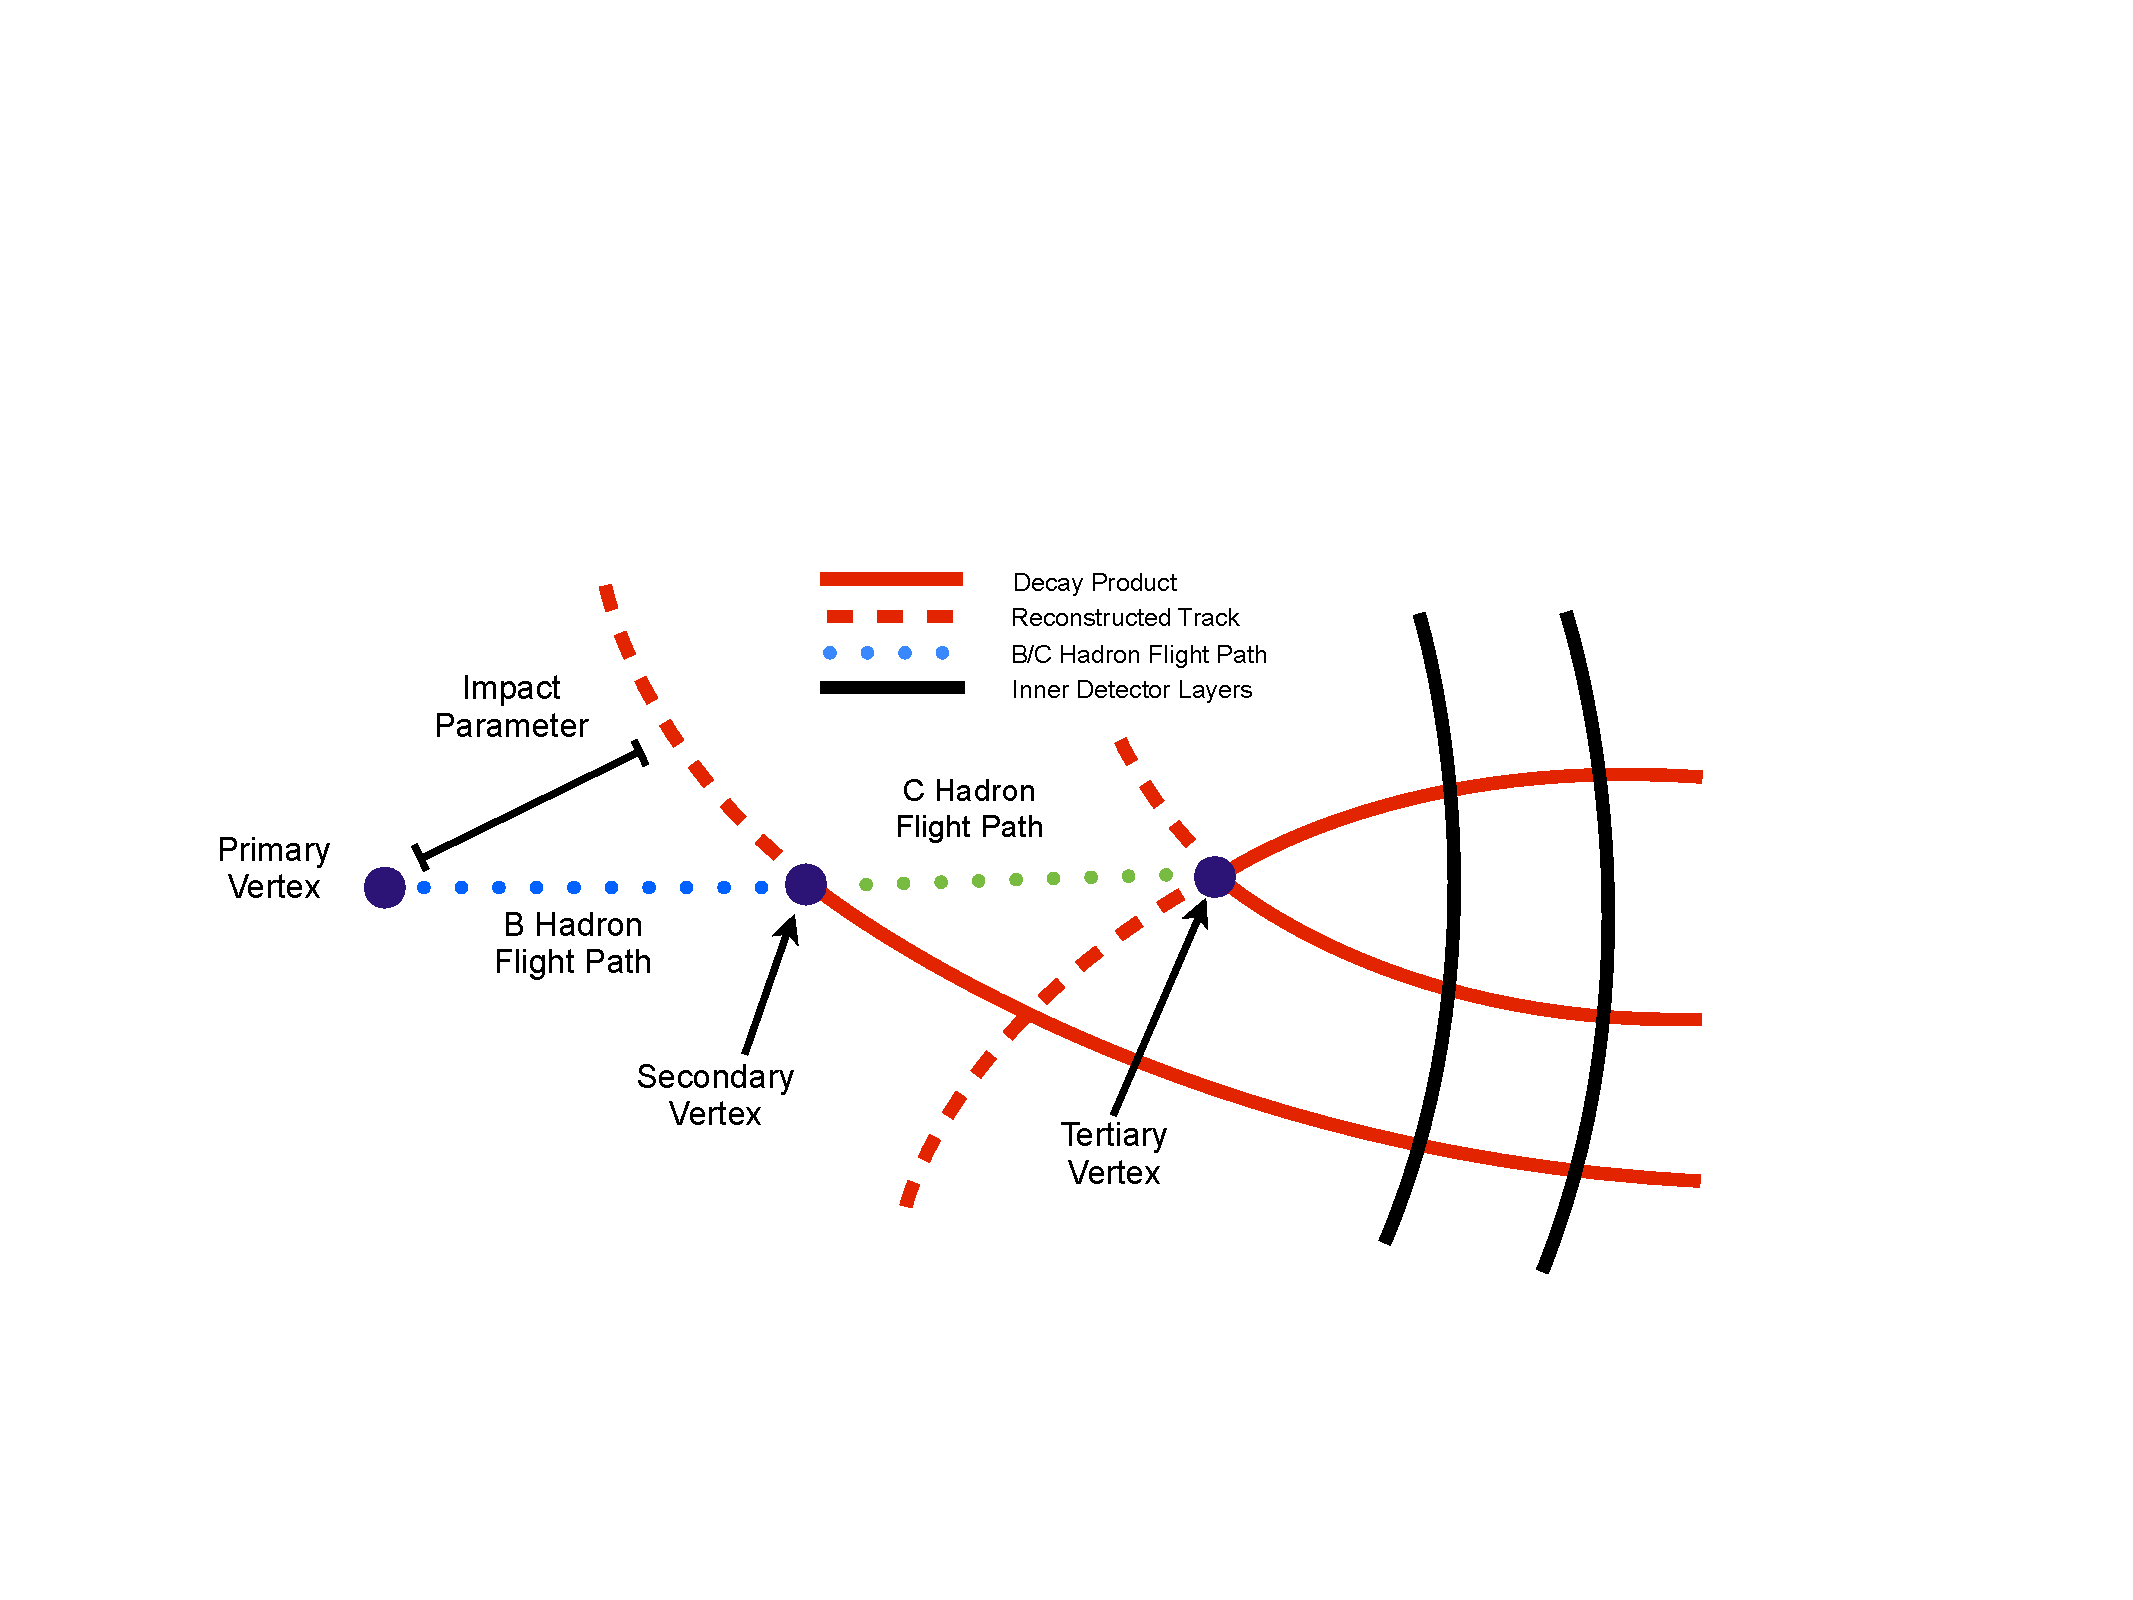
\includegraphics[width=0.85\textwidth]{figs/Objects/bjets_schem_no_beam.pdf}
    \caption
    [The key features of a $b$-jet utilised by the base $b$-tagging algorithms.]
    {An illustration of the key features of a $b$-jet utilised by the base $b$-tagging algorithms.}
    \label{fig:obj_bjets_schem}
  \end{center}
  \vspace{-1cm}
\end{figure}

\subsubsection{Impact Parameter Based Algorithm}
\label{sec:obj-bjets_IP}

The IP3D and IP2D algorithms utilise the impact parameter, which is defined as the shortest distance between a track and the hard-scatter primary vertex.
A track corresponding to a particle from the offset decay vertex of a heavy-hadron is likely to have a large impact parameter,
meaning that the distribution of track impact parameter is different for each of the jet-flavours.
The impact parameter of a track coming from the decay of a heavy hadron is indicated in Figure~\ref{fig:obj_bjets_schem}.
For all tracks associated to a jet, the impact parameter is calculated in both the transverse (perpendicular to beam-line)
and longitudinal (parallel to beam-line) direction, which are referred to as $d_{0}$ and $z_{0}$.
The IP3D algorithm calculates a likelihood of the jet having a specific flavour, 
based on the distributions of the impact parameters ($d_{0}$, $z_{0}$) and their significances ($d_{0}/\sigma _{d0}$ and  $z_{0}/\sigma_{z0}$). 
The IP2D algorithm calculates the jet flavour likelihood from just the transverse distributions, ($d_{0}$ and $d_{0}$ significance), which is more robust to pile-up
because tracks originating from a pile-up primary vertex that occurred at a different position on the $z$-axis are likely to have large $z_{0}$ significance values.


\subsubsection{Secondary Vertex Based Algorithm}
\label{sec:obj-bjets_SV}

The SV1 algorithm aims to reconstruct a secondary vertex of two or more intersecting tracks, corresponding to the decay of a heavy-flavour hadron;
the secondary vertex within a $b$-jet's decay chain is illustrated in Figure~\ref{fig:obj_bjets_schem}.
The SV1 algorithm calculates a set of flavour discriminating variables using the properties of the reconstructed secondary vertex.
Examples of flavour discriminating variables are the invariant mass of tracks associated to a vertex,
which will be larger for $b$-jets due to the heavy mass of the $b$-hadron
\footnote{\ The mass of a $B_0$ or $B^\pm$ meson is $\sim$ 5 GeV, which are the most common $b$-hadrons in a $b$-jet~\cite{obj-bjets_PDG}.}, 
the distance in the transverse plane between the hard-scatter primary vertex and the secondary vertex, % (2D flight path $L_{XY}$),
which will be larger for $b$-jets due to the long lifetime of the $b$-hadron,
and the number of tracks at the secondary vertex, which will be larger for reliable secondary vertices.

\subsubsection{Jet Fitter Algorithm}
\label{sec:obj-bjets_JF}

The JetFitter algorithm (JF) attempts to reconstruct the full decay chain of the $b$-hadron into a $c$-hadron and then into light-hadrons. 
This is done by assuming that all vertices lie on a common $b$-flight axis, and constructing vertices from the intersection of
one or more tracks and the flight axis.
The aim is to reconstruct the secondary and tertiary vertices which correspond to the decays of the $b$ and $c$-hadron,
as illustrated in Figure \ref{fig:obj_bjets_schem}.
Similar to SV1, the JetFitter algorithm then calculates a number of flavour discriminating variables:
for example, vertex mass and number of vertices with two or more tracks.

\subsection{Multi-Variate $b$-Tagging Algorithm}
\label{sec:obj-bjets_MV2}

\begin{figure}[!b]
  \begin{center}
    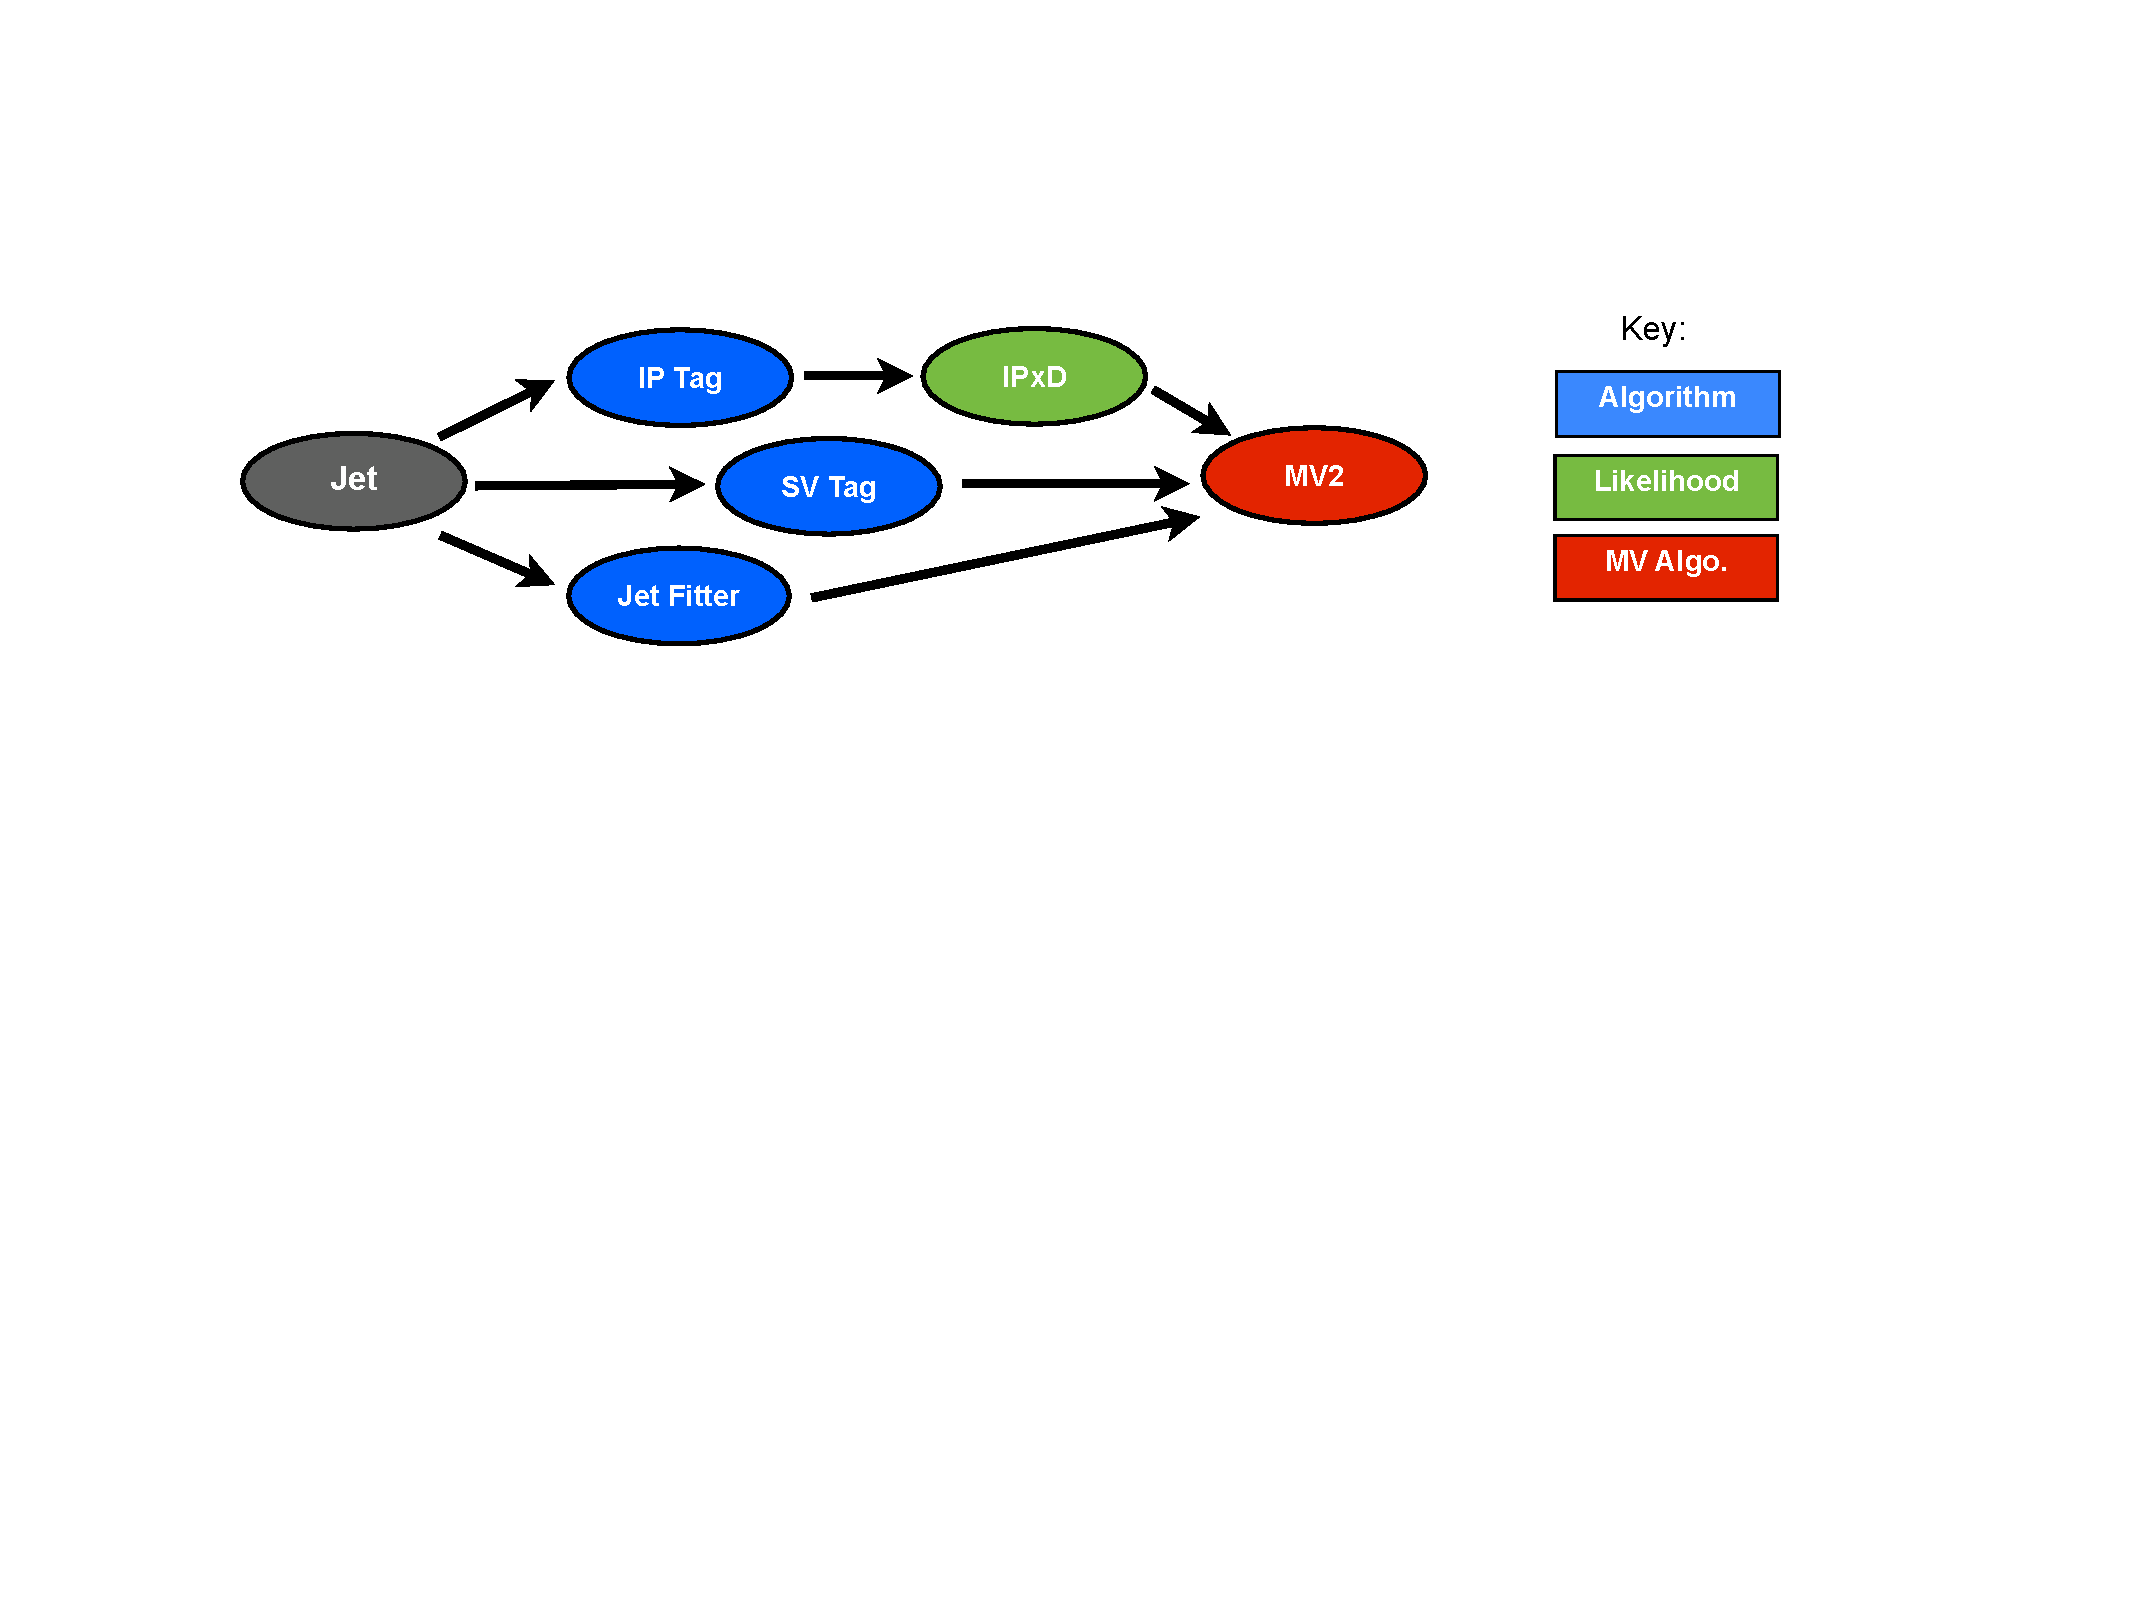
\includegraphics[width=1.0\textwidth]{figs/Objects/MV2_schem.pdf}
    \caption[An illustration of how the three base flavour tagging algorithms are combined in the MV2 algorithm.]
            {An illustration of how the three base flavour tagging algorithms are combined in the MV2 algorithm.
              The figure shows that the flavour discriminating variables from SV1 and Jet Fitter are combined with the likelihood outputs from IP2D and IP3D.}
    \label{fig:obj-MV2_schem}
  \end{center}
  \vspace{-1em}
\end{figure}

The three base algorithms are combined in a Boosted Decision Tree (BDT)~\cite{obj-bjets_bdt},
a machine-learning technique for combining the many flavour discriminating variables, resulting in the MV2 algorithm.
A BDT is able to use the complex correlations between the input variables to maximise $b$-tagging performance.
As shown in Figure~\ref{fig:obj-MV2_schem}, MV2 combines the likelihood output of IP3D and IP2D
with the flavour discriminating variables of SV1 and JF discussed in the preceding sections.
The MV2 output is a variable between -1 and 1, where 1 indicates that the jet is likely to be a $b$-jet and -1 indicates the inverse.

The BDT is trained using a simulated sample of $t\bar{t}$ events that will contain a mix of  $b$-, $c$- and light-jets,
in addition to a sample containing a $Z'$ boson decaying to $b$-quarks to increase statistics in the high jet-\pT{} region.
The training makes use of the truth jet flavour label scheme described in Section~\ref{sec:obj-bjets_label}.
%A training sample with known truth labels is required as this allows the BDT to be optimised
%such that it uses the complex correlations between the input variables to allow for high $b$-jet efficiencies
%whilst still obtaining a large $c$- and light-jet rejection.
Subtly different MV2 algorithms are created using samples containing different fractions of light and $c$-jets;
the fraction of $c$-jets used is labelled in the algorithm name.
For example, the MV2c10 algorithm has been trained on a sample containing 10\% charm-jets, which gives strong light- and $c$-jet rejection.

A $b$-tagged jet is required to have a MV2 output above a specific cut value, such that $b$-tagged jets are likely to be $b$-jets.
The choice of cut value will vary the $b$-jet efficiency, light-jet rejection and $c$-jet rejection: where
$b$-jet efficiency is defined as the probability of $b$-tagging a $b$-jet,
light-jet rejection is defined as 1 divided by the probability of $b$-tagging a light-jet, and
$c$-jet rejection is defined as  1 divided by the probability of $b$-tagging a $c$-jet.
Figure~\ref{fig:obj-bjets_perf} shows the $b$-jet efficiency against (a) light jet rejection and (b) $c$-jet rejection of the MV2 algorithm for a continuous range of cut values.
The different lines show the performance of the algorithm in the 2015 configuration~\cite{obj-bjets_algo_2015}
and in the 2016 configuration~\cite{obj-bjets_algo_2016} where different fractions of $c$-jets are used in the training;
2016 MV2c10 is the configuration used throughout this thesis as recommended in~\cite{obj-bjets_algo_2016}.
    
\vspace{-0.5em}    
\begin{figure}[!ht]
  \begin{center}
    \captionsetup[subfigure]{aboveskip=0pt,justification=centering}
    \subcaptionbox{$b$-jet efficiency \\against light-jet rejection} {\includegraphics[width=0.48\linewidth, angle=0]{figs/Objects/bjets_perf_light.eps}}
    \subcaptionbox{$b$-jet efficiency \\against $c$-jet rejection}  { 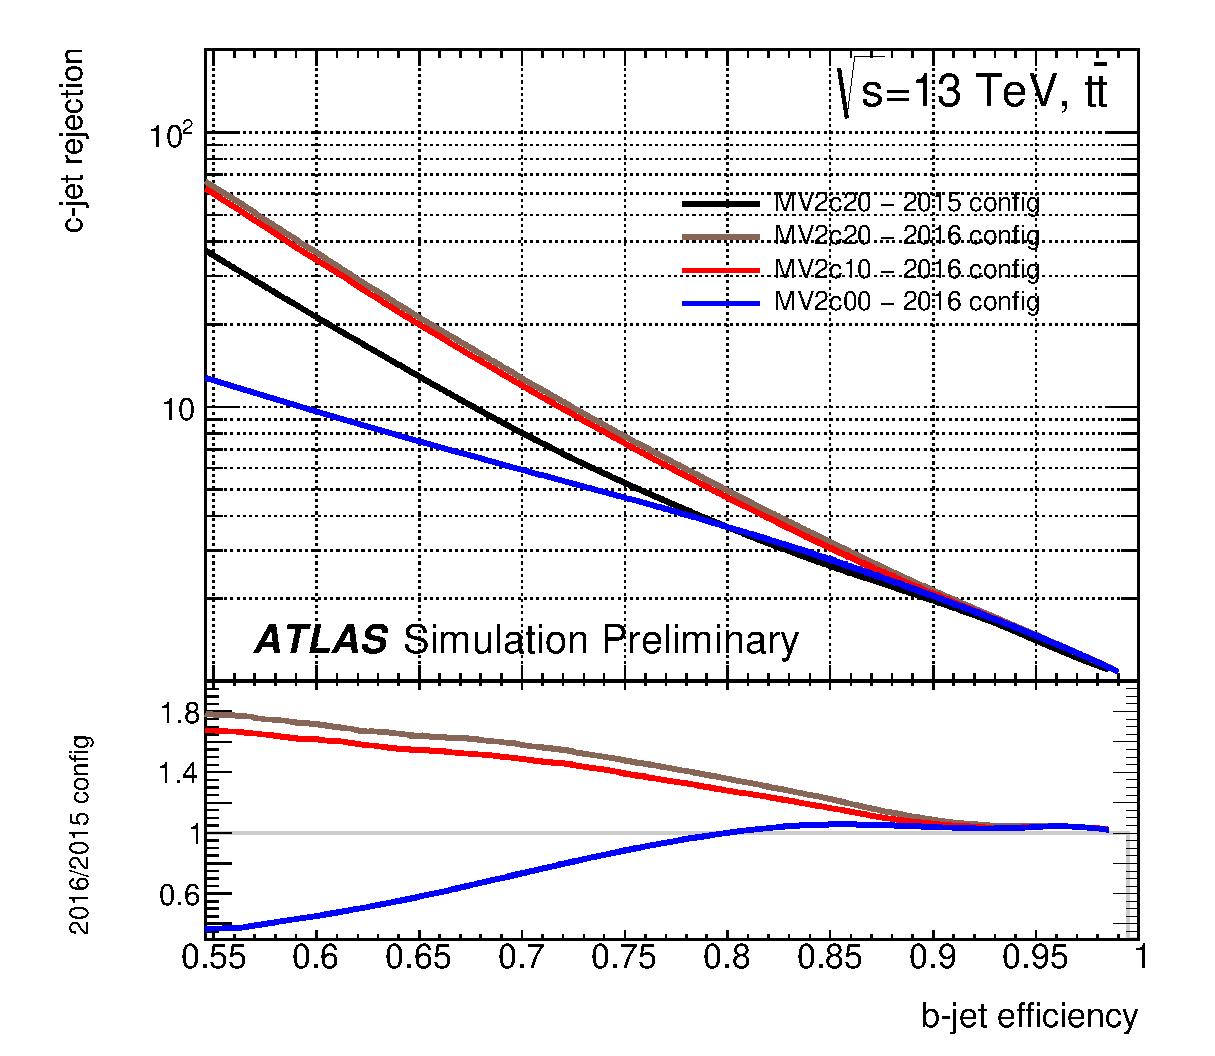
\includegraphics[width=0.48\linewidth, angle=0]{figs/Objects/bjets_perf_charm.eps}}
  \end{center}
  \vspace{-0.5em}
  \caption[The expected $b$-jet efficiency of the $b$-tagging algorithm, MV2, with respect to
    light-jet and $c$-jet rejection in simulated $t\bar{t}$ events.]
    {The expected $b$-jet efficiency of the $b$-tagging algorithm, MV2, with respect to
    (a) light-jet and (b) $c$-jet rejection in simulated $t\bar{t}$ events.
    The various lines show the performance of the algorithm for different configurations and training setups~\cite{obj-bjets_algo_2016}.}
  \label{fig:obj-bjets_perf}
  \vspace{-0.5em}
\end{figure}

There are four standard choices of MV2c10 cut value used in ATLAS analyses,
these standard choices are known as \mbox{$b$-tagging} operating points.
Table~\ref{tab:obj-MV2_WPs} shows the MV2c10 cut value of the four operating points
and the corresponding values of $b$-jet efficiency, $c$-jet rejection, light-jet rejection and $\tau$ rejection
measured using simulated $t\bar{t}$ events for jets with $\pT$ greater than 20 GeV.

\begin{table}[!htb]
\vspace{-0.5em}
\begin{center}
    \begin{tabular}{|c||c|c|c|c|}
      \hline
      MV2c10 Cut Value  &  $b$-jet efficiency   &     $c$-jet rejection   &   Light-jet rejection  &    $\tau$ rejection  \\
      \hline
      0.9349         &           60\%             &           34          &      1538              &     184              \\
      0.8244         &           70\%             &           12          &       381              &      55              \\
      0.6459         &           77\%             &           6           &       134              &      22              \\
      0.1758         &           85\%             &           3.1         &        33              &     8.2              \\
      \hline
    \end{tabular}
    \caption[The MV2c10 $b$-tagging algorithm operating points; with the corresponding $b$-jet~efficiency, $c$-jet~rejection, light-jet~rejection and $\tau$~rejection.]
            {The MV2c10 $b$-tagging algorithm operating points; with the corresponding $b$-jet~efficiency, $c$-jet~rejection, light-jet~rejection and $\tau$~rejection.
             These values have been derived using simulated $t\bar{t}$ events for jets with \pT{} above 20 GeV~\cite{obj-bjets_algo_2016}.}
            \label{tab:obj-MV2_WPs}
  \end{center}
  \vspace{-2em}
\end{table}

The $b$-jet efficiencies given in Table~\ref{tab:obj-MV2_WPs} are used to name the corresponding $b$-tagging operating points,
as such the operating points are known as the 60\%, 70\%, 77\% and 85\% \mbox{$b$-tagging} operating points.
To be specific, for a jet to be $b$-tagged at the 70\% operating point
the output of the MV2c10 algorithm performed on that jet must be greater than 0.8244.


$b$-tagging performance is known to decrease at high jet-\pT{}.
To illustrate this trend, Figure~\ref{fig:obj-bjets_perf_pt} shows the $b$-tagging efficiency for $b$-jets, $c$-jets and light-jets in $t\bar{t}$ simulation as a function of jet-\pT{}
for the MV2c20 algorithm in the 2015 configuration~\cite{obj-bjets_algo_2015}. A similar trend is also found for the MV2c10 using the 2016 configuration~\cite{obj-bjets_algo_2016}.

\begin{figure}[!htb]
  \vspace{-0.5em}
\begin{center}
    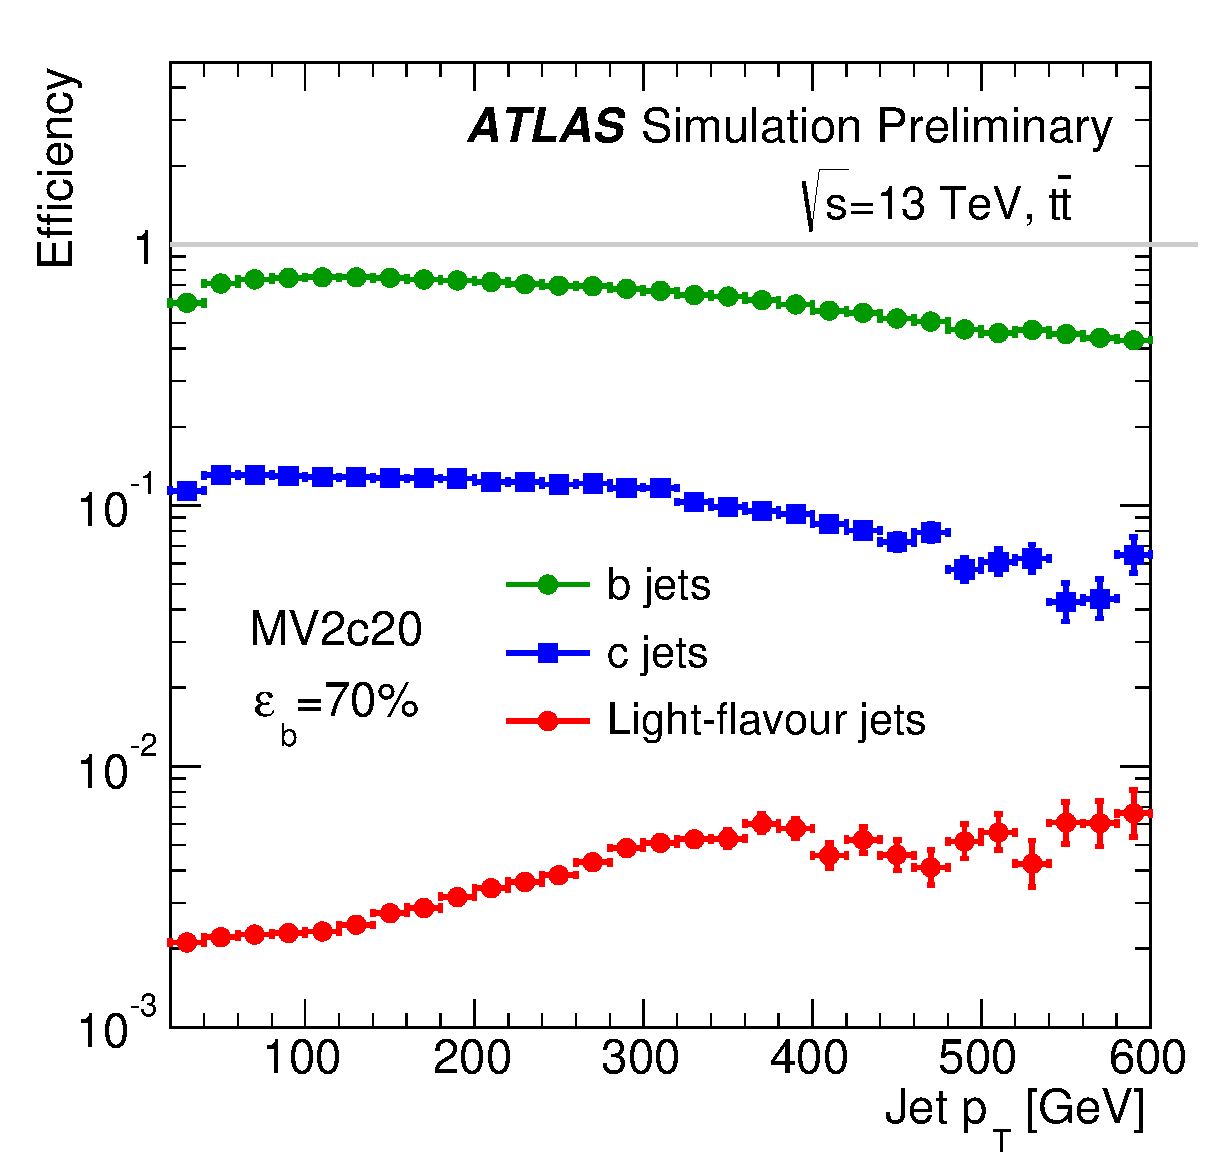
\includegraphics[width=0.48\linewidth, angle=0]{figs/Objects/bjets_perf_pt.eps} 
  \end{center}
  \vspace{-1em}
  \caption[The $b$-tagging efficiency for $b$-jets, $c$-jets and light-jets as a function of jet-\pT{} for the MV2c20 algorithm at the 70\% operating point in the 2015 configuration.]
          {\label{fig:obj-bjets_perf_pt}The $b$-tagging efficiency for $b$, $c$ and light-jets against jet-\pT{} 
            for the MV2c20 algorithm at the 70\% operating point using the 2015 configuration in simulated $t\bar{t}$ events~\cite{obj-bjets_algo_2015}.}
\vspace{-1em}
\end{figure}

The decrease $b$-tagging performance at high $p_T$ is due to a number of factors.
Firstly, high-\pT{} jets are more collimated meaning that reconstructed vertices
will have a larger positional uncertainty and fake vertices become more common.
Secondly, the fraction of tracks in a $b$-jet that do not come from the decay of a $b$-hadron increases,
meaning that the flavour discriminating variables are diluted.
Finally, at high-\pT{} the $b$-hadron can decay on the far side of the IBL, leading to a reduced vertex and impact parameter resolution.


\subsection{Calibration and Uncertainties}
\label{sec:obj-bjets_calib}

A calibration is performed to correct the modelling of $b$-tagging in simulation to the $b$-tagging performance in data.
The $b$-tagging calibration uses di-lepton $t\bar{t}$ events which, as described in Section~\ref{sec:theo-ttbar},
have a distinctive signature for event selection and provide a high-purity sample of $b$-jets~\cite{obj-bjets_calib_tech,obj-bjets_calib_plots}.
From the high-purity $b$-jet sample one can perform a likelihood fit to extract the $b$-jet efficiency, $\epsilon_{\,b\text{Tag}}$, which is defined as:
\begin{equation}
 \epsilon_{\,b\text{Tag}} = \frac{N(\text{$b$-tagged $b$-jets)}}{N(\text{$b$-jets)}}
\end{equation}
where $b$-tagged means above the cut on the MV2 output for a given operating point.
By measuring $\epsilon_{\,b\text{Tag}}$ in both data and in Monte-Carlo simulation one can derive
a correction to simulation, known as a data/simulation scale factor ($SF_{\,b\text{Tag}}$):
\begin{equation}
 SF_{\,b\text{Tag}} = \epsilon_{\,b\text{Tag}}^{\text{Data}}/\epsilon_{\,b\text{Tag}}^{\text{MC}}
\end{equation}
Uncertainties are derived for the scale factors 
to account for uncertainties in the modelling of the Standard Model processes and the detector response to electrons, muons and jets in simulation.
The dominant source of uncertainty is the modelling of $t\bar{t}$ in simulation.
Figure~\ref{fig:obj-bjets_calib} shows the data/simulation scale factor measured in 2015 and 2016 data as a function of jet \pT{}.
%The scale factors are consistent with unity within uncertainties, showing that $b$-tagging is generally well-modelled in simulation.

\begin{figure}[!ht]
  \begin{center}
  \vspace{-1em}
    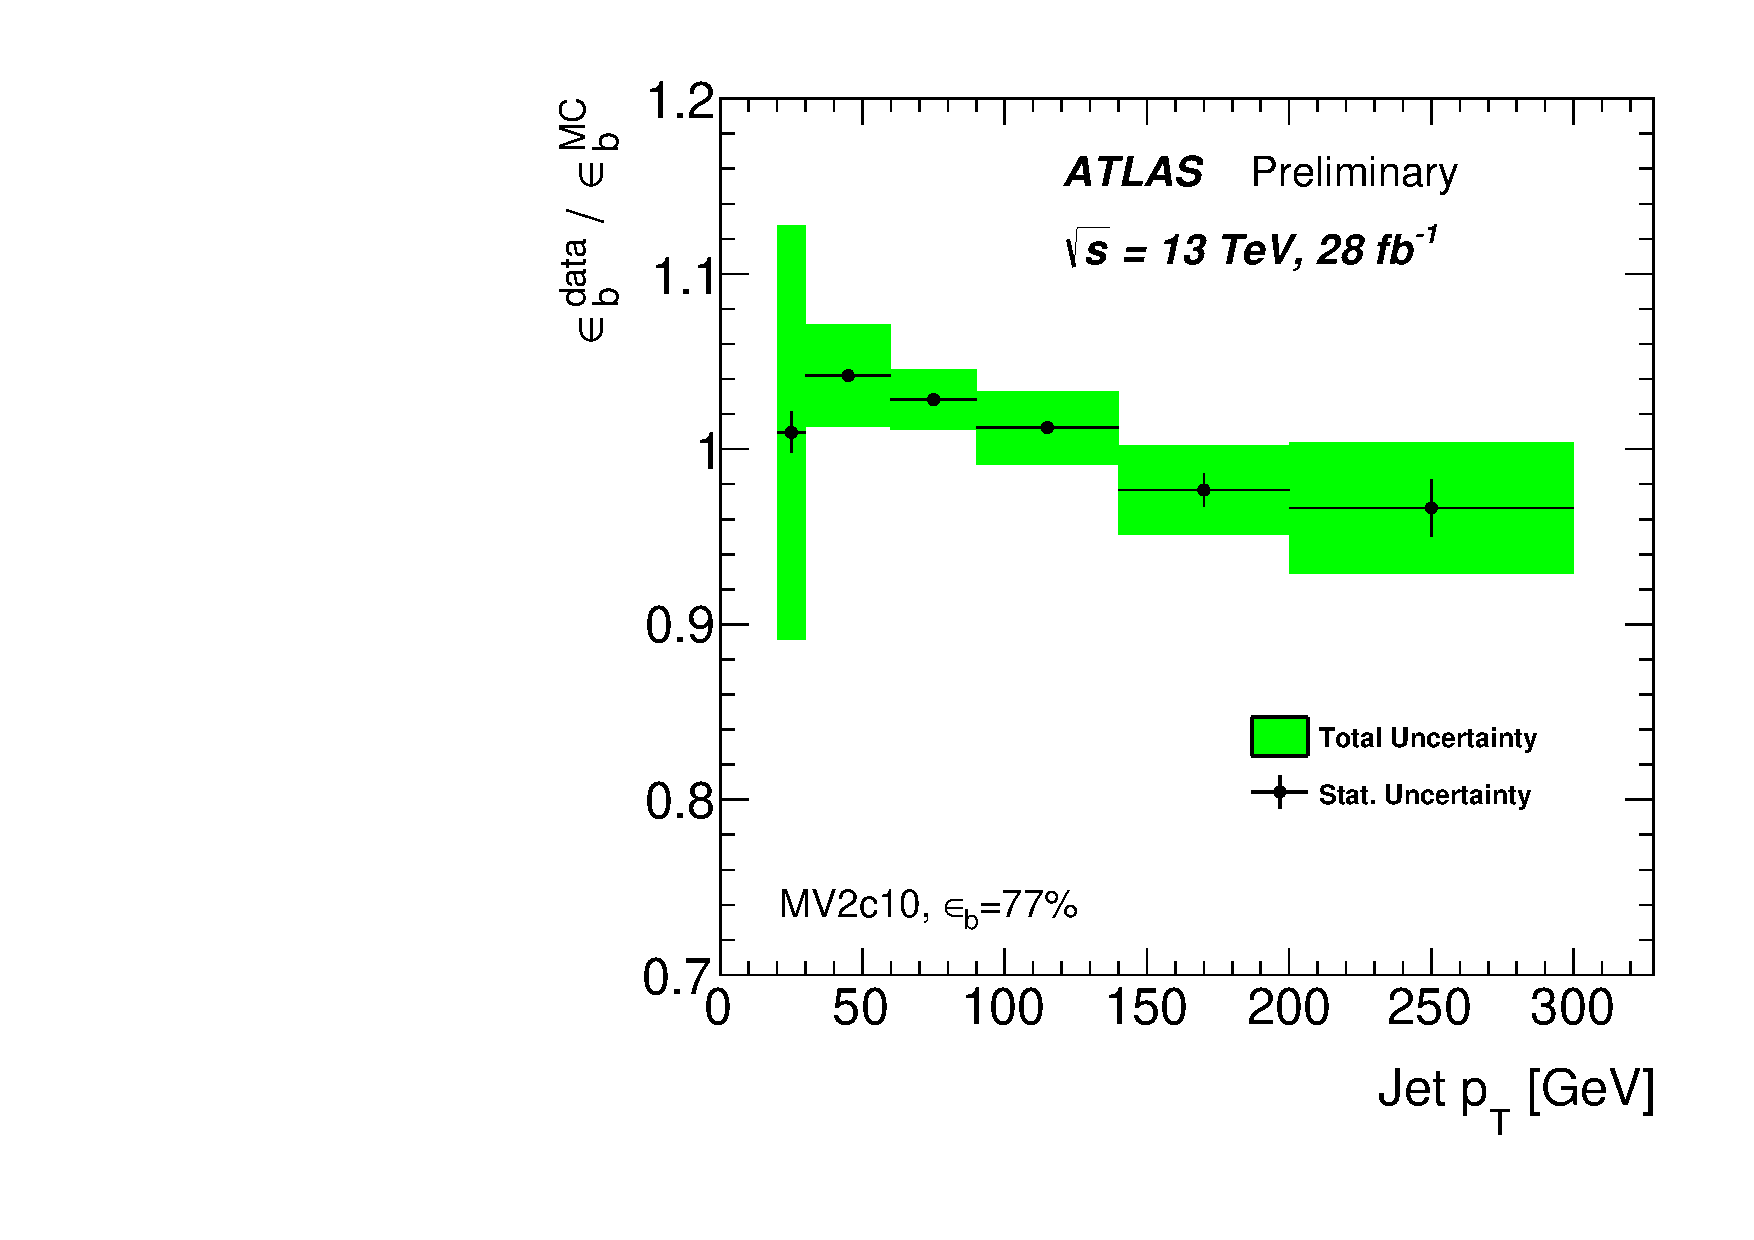
\includegraphics[width=0.55\linewidth, angle=0]{figs/Objects/bjets_calib_pt.pdf} 
  \end{center}
  \vspace{-1.3em}
  \caption[The ratio of $b$-tagging efficiency in data and simulation for MV2c10 at the 77\% operating point as a function of jet-\pT{} in di-lepton $t\bar{t}$ events.]
          {\label{fig:obj-bjets_calib}The ratio of $b$-tagging efficiency in data and Monte Carlo for MV2c10 at the 77\% operating point as a function of jet-\pT{}
  in di-lepton $t\bar{t}$ events. Statistical uncertainties (black lines) and total uncertainties (green shaded region) are shown \cite{obj-bjets_calib_plots}.}
\end{figure}

The $b$-tagging calibration using di-lepton $t\bar{t}$ events described above
is unable to measure a data/simulation scale factor for jets with \pT{} greater than 300 GeV, due to low data statistics in the high-\pT{} region.
Thus, the measured scale factors are extrapolated to cover the high jet-\pT{} region.
To derive an uncertainty for the high-\pT{} extrapolation; $\epsilon_{\,b\text{Tag}}$ is measured in Monte-Carlo simulations of high-\pT{} $b$-jets  
when variables known to affect the performance of $b$-tagging are varied to represent the modelling uncertainties of high-\pT{} \mbox{$b$-jets}~\cite{obj-bjets_calib_highPt}.
The dominant extrapolation uncertainty is from variations of the impact parameter resolution.

\subsection{$b$-Jet Energy Scale}
\label{sec:obj-bjets_bjes}

Section~\ref{sec:obj-jets_calib} described the
jet energy scale correction applied to hadronic jets.
For $b$-jets this correction may be different due to differences in the parton shower and hadronisation processes for a $b$-jet;
for example, during the decay of the $b$-hadron, muons and neutrinos can be produced that will not deposit all/any of their energy in the calorimeter.

%As a result, an additional $b$-jet energy scale ($b$JES) uncertainty has been 
%specifically derived in a previous di-$b$-jet search at ATLAS~\cite{dibjet-mori16_paper}.
%Figure~\ref{fig:obj-bjets_bJES_uncert} shows the derived total $b$JES uncertainty with respect to jet-\pT{},
%the components that contribute to the uncertainty are also shown.
%The contributions to the $b$JES uncertainty considered are $b$-jet modelling in simulation (referred to as fragmentation),
%modelling of the detector response (material description), $b$-tagging calibration and jet energy resolution.
%In addition, an uncertainty is applied to cover a bias in the number of charged tracks associated to a $b$-jet with respect to a light jet,
%which is necessary because, as is described below, tracks are used to validate the $b$JES uncertainty.
%
%
%\begin{figure}[!hbt]
% \vspace{-1em}  
%  \begin{center}
%    \includegraphics[width=0.53\linewidth, angle=0]{figs/Objects/bjets_bJES_uncert_edit.pdf}
%  \vspace{-2em}
%  \end{center}
%  \caption[The total fractional $b$-jet energy scale uncertainty shown with the contributions from the various sources of uncertainty.]
%          {\label{fig:obj-bjets_bJES_uncert} The total fractional $b$-jet energy scale uncertainty
%          shown with the contributions from the various sources of uncertainty~\cite{dibjet-int_mori16}.}
%\end{figure}

As a result, an additional $b$-jet energy scale ($b$JES) uncertainty has been 
specifically derived in a previous di-$b$-jet search at ATLAS~\cite{dibjet-mori16_paper}.
The $b$JES uncertainty is found to be within 2.6\% for all jets with a \pT{} greater than 60~\GeV.
The dominant source of the $b$JES uncertainty is from the 
modelling of the detector response to $b$-jets in simulation;
other contributions to the $b$JES uncertainty considered are
the modelling of $b$-jet formation in simulation,
$b$-tagging calibration and jet energy resolution.
In addition, an uncertainty is applied to cover a bias in the number of charged tracks associated to a $b$-jet with respect to a light jet,
which is necessary because, as is described below, tracks are used to validate the $b$JES uncertainty.

The $b$JES uncertainty is validated by comparing jet energy measurements to independently calibrated objects, in this case tracks that are associated to the jets.
It is found that the energy of $b$-tagged jets is consistent with the energy of jets with no $b$-tagging applied
within the 2.6\% $b$JES uncertainty considered. Therefore no additional $b$JES correction is required.

\vfill
\newpage
\section{Electrons and Muons}
\label{sec:obj-leptons}

Reconstruction of electrons and muons
is important for a number of analyses at ATLAS;
including the selection of di-lepton $t\bar{t}$ events
which is used in the calibration of  the $b$-jet trigger,
described in Section~\ref{sec:trig-bjet_eff}.
%As these objects are not used in the final analysis presented in this thesis,
%they are described below in less detail than has been given to jets and $b$-jets.

Electron~\footnote{\ For the purposes of reconstruction positrons are included as a subset of electrons.}
reconstruction at ATLAS ~\cite{obj-electrons} uses
the matching of narrow clusters of energy deposits in the EM calorimeter
to a track from the ID (described in Section~\ref{sec:obj-tracks}),
from which the four-momentum of the electron can be determined.
Information such as the calorimeter shower shape,
properties of the matched track
and TRT transition radiation (described in Section~\ref{sec:det-ID})
are used to identify electrons.
Three different operating points are provided for electron identification
which are, in order of increasing background rejection:
\textit{Loose}, \textit{Medium} and \textit{Tight}. 

Muons~\footnote{\ Similar to positrons, in reconstruction anti-muons are included as a subset of muons.}
are the only charged particle not to be stopped by the ATLAS calorimeter.
Therefore muons are identified at ATLAS using hits in the sub-detector outside of the calorimeter, the Muon Spectrometer (MS), which is described in Section~\ref{sec:det-MS}.
Two of the techniques used for muon reconstruction are combined muons and extrapolated muons.
Combined muons are reconstructed by extrapolating tracks formed in the MS inwards to match tracks formed in the ID;
if a match is found then a muon track is reconstructed from the associated ID and MS hits.
By using both ID and MS hits, a higher precision muon track is created
and the muon tracks can be accurately assigned to a primary vertex, which is used to identify muons from pile-up.
Extrapolated muons are muon tracks formed using only hits in the MS
with a loose requirement on the track pointing to the hard-scatter primary vertex to reduce effects from pile-up;
extrapolated muons are important in the range $2.5 < |\eta| < 2.7$ for which there is no ID coverage.
The four-momentum of the reconstructed muons is determined from the direction and curvature of the muon tracks.

The muon identification operating points are \textit{Loose}, \textit{Medium}, \textit{Tight} and \textit{High-\pT{}}.
Medium muons, used in Section~\ref{sec:trig-bjet_eff}, are combined or extrapolated muons that pass a quality criteria based on
number of MS hits, track fit quality and, where relevant, compatibility between the ID and MS tracks.

%\section{Further objects}
%\label{sec:obj-further}
%
%In this chapter all objects used in the analyses presented in this thesis have been defined.
%However there are more objects that ATLAS can reconstruct, a subset of which are briefly outlined below.
%\textit{`Photons'} are identified using narrow clusters of energy deposits in the calorimeter similar to that of electrons,
%  except with no track associated~\cite{obj-photons}. %\vspace{em}
% Hadronically decaying \textit{`taus'} are identified and reconstructed using narrow calorimeter jets
% associated to a topologies of tracks that match their known decay chain~\cite{obj-taus}.
% \textit{`Missing Transverse Momentum'} (MET) is the negative sum of the transverse momenta of all reconstructed physics objects in an event~\cite{obj-met}.
% As momentum is conserved in the transverse plane, MET measures the sum of the $p_T$ of objects that did not interact with the ATLAS detector.
%  MET is used to identify neutrinos~\cite{obj-Hbb} and to search for dark matter~\cite{obj-met_monoJet}.
%\end{itemize}
